\chapter{Kerr black hole}
\label{s:ker}
\index{Kerr!black hole}

\minitoc

\section{Introduction}

\section{The Kerr solution}

\subsection{Expression in Boyer-Lindquist coordinates} \label{s:ker:expr_BL}

The Kerr solution depends on two constant non-negative real parameters:
\begin{itemize}
\item the \defin{mass parameter}\index{mass!parameter of Kerr solution} $m > 0$, to be
interpreted in Sec.~\ref{s:ker:Komar_mass} as the spacetime total mass;
\item the \defin{spin parameter}\index{spin!parameter of Kerr solution} $a \geq 0 $,
to be interpreted in Sec.~\ref{s:ker:Komar_J} as the reduced angular momentum  $a=J/m$, $J$ being the
spacetime total angular momentum.
\end{itemize}
In this part, we focus on Kerr solutions for which
\be \label{e:ker:a_lower_m}
    0 < a < m .
\ee
The Kerr solution is usually presented in the so-called
\defin{Boyer-Lindquist coordinates}\index{Boyer-Lindquist coordinates}
$(t,r,\th,\ph)$. Except for the standard singularities of the
spherical coordinates $(\th,\ph)$ on $\SS^2$ at $\theta\in\{0,\pi\}$,
we may consider that the Boyer-Lindquist coordinates cover the manifold
$\R^2\times\SS^2$, with $t$ spanning $\R$, $r$
spanning\footnote{This contrasts with $r$ spanning only $(0,+\infty)$ for
the standard spherical coordinates $(r,\th,\ph)$ on $\R^3$.} $\R$ and
$\th$ spanning $(0,\pi)$ and $\ph$ spanning $(0,2\pi)$. Hence
$(t,r)$ is a Cartesian chart covering $\R^2$ and $(\th,\ph)$ is the standard
spherical chart of $\SS^2$.

\begin{figure}
\centerline{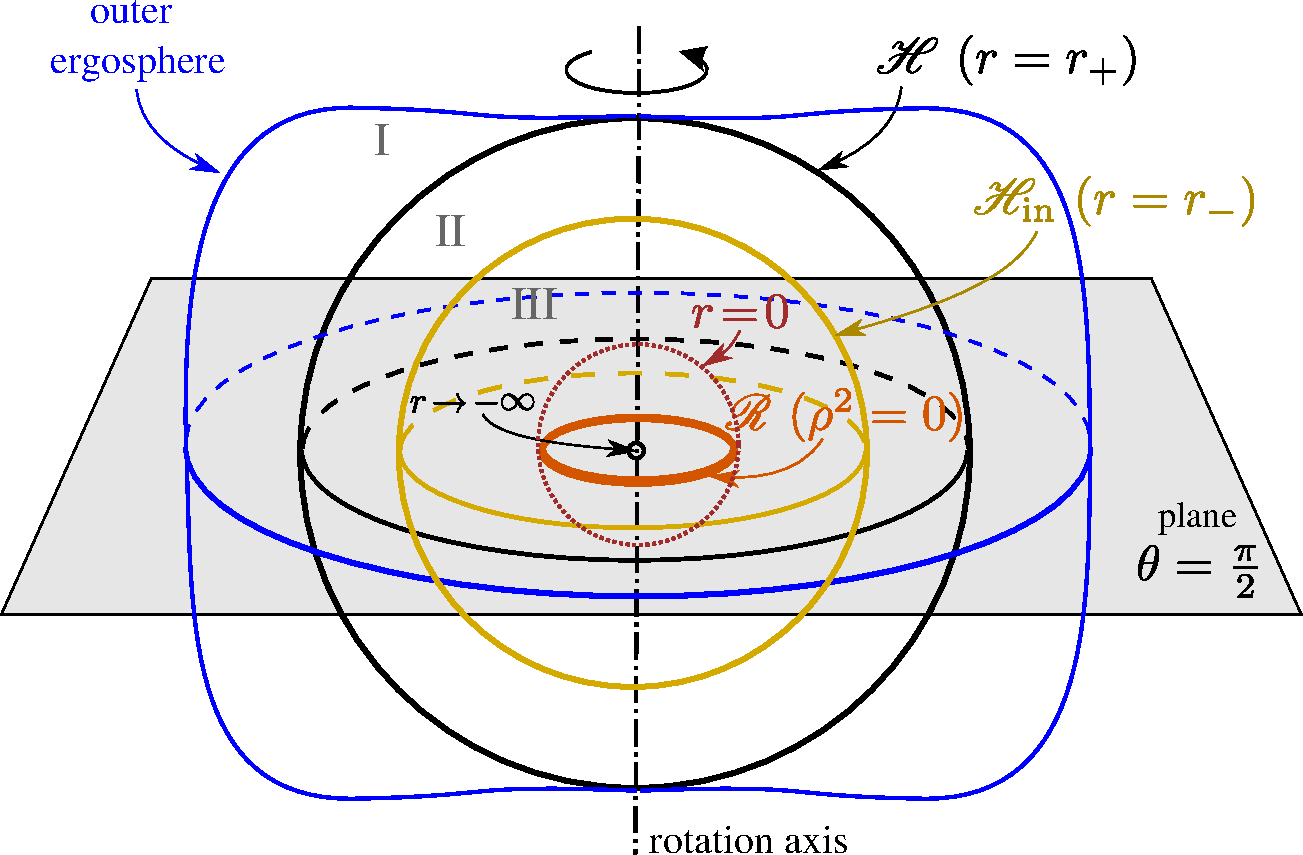
\includegraphics[width=0.8\textwidth]{ker_spher_view.pdf}}
\caption[]{\label{f:ker:spher_view} \footnotesize
View of a section $t=\mathrm{const}$ of $\mathbb{R}^2\times\mathbb{S}^2$
in terms of the coordinates $(R,\th,\ph)$, with $R:=\mathrm{e}^r$,
so that the region $r\rightarrow -\infty$
is reduced to a single point at the centre of all the pictured spheres.
Such coordinates have been introduced for picturial purposes by O'Neill
\cite{ONeil95}.}
\end{figure}


In this section, let us choose the spacetime manifold to be the open subset $\M_{\rm BL}$
of $\mathbb{R}^2\times\mathbb{S}^2$ formed by the disjoint union of
the following three components (cf. Fig.~\ref{f:ker:spher_view}):
\begin{subequations}
\begin{align}
    \M_{\rm BL} & :=  \M_{\rm I} \cup \M_{\rm II} \cup \M_{\rm III} , \\
    \M_{\rm I} & :=  \R\times(r_+,+\infty)\times\SS^2 \label{e:ker:def_M_I}\\
    \M_{\rm II} & :=  \R\times(r_-,r_+)\times\SS^2 \\
    \M_{\rm III} & :=  \R\times(-\infty,r_-)\times\SS^2 \setminus \ring, \label{e:ker:def_M_III}
\end{align}
\end{subequations}
where
\be \label{e:ker:def_r_pm}
    \encadre{r_+ := m + \sqrt{m^2-a^2}} \quad\mbox{and}\quad  \encadre{r_- := m - \sqrt{m^2-a^2}}
\ee
and $\ring$ is the subset of $\R^2\times\SS^2$ defined in terms of the Boyer-Lindquist coordinates $(t,r,\th,\ph)$ by
\be \label{e:ker:def_ring}
    \ring = \left\{ p \in \R^2\times\SS^2,
        \quad r(p) = 0 \ \mbox{and}\ \th(p) = \frac{\pi}{2} \right\} .
\ee
Note that thanks to the constraint (\ref{e:ker:a_lower_m}), $r_+$ and $r_-$
are well defined and obey
\be
    0 < r_- < m < r_+ < 2 m .
\ee
Note also that $\ring$ is spanned by the coordinates $(t,\ph)$ and is diffeomorphic to the 2-dimensional cylinder $\R\times\SS^1$:
\be \label{e:ker:ring_R_S1}
    \ring \simeq \R\times\SS^1 .
\ee
This is so because $r=0$ is \emph{not} a peculiar value of $r$ in $\R^2\times\SS^2$
(cf. Fig.~\ref{f:ker:spher_view}).
In view of Eqs.~(\ref{e:ker:def_M_I})-(\ref{e:ker:def_M_III}) and (\ref{e:ker:def_ring}), it is clear that
the various connected components of $\M_{\rm BL}$ are defined in terms of the
Boyer-Lindquist coordinates $(t,r,\th,\ph)$ by
\begin{subequations}
\label{e:ker:M_I_III_r}
\begin{align}
  \forall p \in  \M_{\rm BL},\quad p \in \M_{\rm I} & \iff r(p) > r_+ \\
    \quad p \in \M_{\rm II} & \iff r_- < r(p) < r_+ \\
    \quad p \in \M_{\rm III} & \iff r(p) < r_-\ \mbox{and}\
    \left( r(p) \not=0 \ \mbox{or}\ \theta(p) \not=\frac{\pi}{2} \right) .
\end{align}
\end{subequations}


The \defin{Kerr metric}\index{Kerr!metric} is defined by the following
components in terms of the Boyer-Lindquist coordinates $(t,r,\th,\ph)$:
\be \label{e:ker:metric_BL}
    \encadre{
    \begin{array}{ll}
    g_{\mu\nu}\,  \D x^\mu \D x^\nu  = &
    \displaystyle - \left( 1 - \frac{2m r}{\rho^2} \right) \, \D t^2
    - \frac{4 a m  r \sin^2\th}{\rho^2} \,  \D t\, \D\ph
    + \frac{\rho^2}{\Delta} \, \D r^2  \\[2ex]
    & \displaystyle + \rho^2 \D \th^2
    + \left( r^2 + a^2 + \frac{2 a^2 m r \sin^2\th}{\rho^2} \right)
    \sin^2\th \, \D \ph^2 ,
    \end{array}
    }
\ee
with
\be \label{e:ker:def_rho2}
    \encadre{\rho^2 := r^2 + a^2 \cos^2\th}
\ee
and
\be \label{e:ker:def_Delta}
    \encadre{\Delta := r^2 - 2 m r + a^2 = (r-r_-)(r-r_+)} .
\ee
Note that on $\M_{\rm BL}$, $\rho\not=0$ and $\Delta\not=0$ (by construction
of $\M_{\rm BL}$!), so that the metric components (\ref{e:ker:metric_BL})
are regular in $\M_{\rm BL}$, except for the standard singularities of
the spherical coordinates $(\th,\ph)$.

By means of a computer algebra system (cf. Sec.~\ref{s:sam:Kerr_solution}),
it is easy to check that
\begin{greybox}
$\left(\M_{\rm BL},\w{g}\right)$ with $\w{g}$ given
by (\ref{e:ker:metric_BL}), is a solution of Einstein equation (\ref{e:bas:Einstein_eq})
in vacuum ($\w{T}=0$) and with a vanishing cosmological constant ($\Lambda=0$).
\end{greybox}

\subsection{Basic properties} \label{s:ker:basic_prop}

Various properties of the Kerr metric are immediate:
\begin{itemize}
\item For $r\rightarrow+\infty$ or $r\rightarrow-\infty$, one has $\rho^2\sim r^2$ and
$\rho^2/\Delta \sim (1-2m/r)^{-1}$,
and $4 a m  r / \rho^2\,  \D t\, \D\ph \simeq 4 a m/r^2 \,  \D t\, r\D\ph$,
so that the metric (\ref{e:ker:metric_BL}) becomes
\be \label{e:ker:asympt_metric}
    g_{\mu\nu}\,  \D x^\mu \D x^\nu  \simeq  - \left( 1 - \frac{2m}{r} \right) \, \D t^2
    + \left( 1 - \frac{2m}{r} \right) ^{-1} \D r^2
    + r^2 \left( \D \th^2 + \sin^2\th  \, \D \ph^2 \right)
    + O\left(\frac{1}{r^2}\right)
\ee
For $r>0$, we recognize the Schwarzschild metric\index{Schwarzschild!metric} expressed
in Schwarzschild-Droste coordinates [cf. Eq.~(\ref{e:sch:Schwarz_metric_SD})].
For $r<0$, the change of coordinate $r'=-r$ leads also to the Schwarzschild metric
but with a negative mass parameter $m'=-m$.
Hence, the Kerr metric has (at least) two asymptotically flat ends: one in
$\M_{\rm I}$ for $r\rightarrow + \infty$ and one in $\M_{\rm III}$ for
$r\rightarrow - \infty$.
\item Since in (\ref{e:ker:metric_BL}) all the metric components $g_{\alpha\beta}$ are independent from $t$ and $\ph$, the
spacetime $(\M_{\rm BL},\w{g})$ admits two isometries, generated by the Killing
vectors
\be
    \encadre{\w{\xi} := \wpar_t} \quad\mbox{and}\quad
    \encadre{\w{\eta} := \wpar_\ph}.
\ee
Since $t$ spans $\R$, the isometry group generated by $\w{\xi}$ is clearly
the translation group\index{translation!group}\index{group!translation --} $(\R,+)$. Moreover, in
view of (\ref{e:ker:asympt_metric}), we have $\w{\xi}\cdot\w{\xi} = g_{tt} < 0$
as $r\rightarrow +\infty$, which means that the Killing vector $\w{\xi}$
is asymptotically timelike. Given the definition of stationarity stated in
Sec.~\ref{s:sta:def_station}, we conclude that the Kerr spacetime is
stationary.
On the other side, since $\ph$ is an azimuthal coordinate
on $\SS^2$, the isometry group generated by $\w{\eta}$ is the rotation
group\index{rotation!group}\index{group!rotation --} $\mathrm{SO}(2) = \mathrm{U}(1)$.
Hence, the Kerr spacetime is axisymmetric.
\item When $a\not=0$, as we have assumed in (\ref{e:ker:a_lower_m}), the
Kerr spacetime is not static, since the stationary Killing vector $\w{\xi}$
is not orthogonal to the hypersurfaces $t=\mathrm{const}$. Indeed
from (\ref{e:ker:metric_BL}),
\[
    a\not=0 \ \Longrightarrow \ \w{\xi}\cdot\w{\eta} = g_{t\ph} \not=0 ;
\]
since $\w{\eta}$ is tangent to the hypersurfaces $t=\mathrm{const}$, this implies
that $\w{\xi}$ is not normal to these hypersurfaces.
\item When $a\rightarrow 0$, we have $r_+\rightarrow 2m$, $r_-\rightarrow 0$,
$\rho^2\sim r^2$, and $\rho^2/\Delta \sim (1-2m/r)^{-1}$, and we see on
(\ref{e:ker:metric_BL}) that the Kerr metric reduces to the Schwarzschild metric.
\item On the hypersurface $r=0$, we have $\rho^2=a^2\cos^2\th$ and $\Delta=a^2$, so that the Kerr metric (\ref{e:ker:asympt_metric}) induces the metric:
\be \label{e:ker:metric_r0}
    h_{ij} \, \D x^i \D x^j = - \D t^2 + a^2\left( \cos^2\th \,  \D \th^2 + \sin^2\th \, \D \ph^2 \right) ,
\ee
where $x^i=(t,\th,\ph)$. According to the assumption (\ref{e:ker:a_lower_m}), $a\not=0$
and the change of coordinates  $x:=a\sin\th\cos\ph$, $y:=a\sin\th\sin\ph$
turns the right-hand side of (\ref{e:ker:metric_r0}) into $- \D t^2 + \D x^2 + \D y^2$.
We recognize a \emph{flat} Minkowskian metric. In particular, for a fixed value
of $t$, the $r=0$ ``sphere'' $\mathcal{S}_t = \{p\in \M_{\rm III}, r(p)=0, t(p)=t\}$
(pictured by the dotted line in Fig.~\ref{f:ker:spher_view})
is made of two disconnected components, which are two \emph{flat open disks} of radius $a$, corresponding respectively to $\theta < \pi/2$ and $\theta>\pi/2$.
\end{itemize}

\subsection{Determinant and inverse metric}

The determinant of the metric $\w{g}$ with respect to Boyer-Lindquist coordinates
is deduced from (\ref{e:ker:metric_BL}); it takes a
relatively simple form (cf. Sec.~\ref{s:sam:Kerr_solution} for the computation):
\be
    \det (g_{\alpha\beta}) = - \rho^4 \sin^2\th .
\ee

The inverse metric is (cf. Sec.~\ref{s:sam:Kerr_solution} for the computation)
\be \label{e:ker:inv_met_BL}
    g^{\alpha\beta} = \left(
    \begin{array}{cccc}
    - \frac{1}{\Delta}
    \left( r^2 + a^2 + \frac{2 a^2 m r \sin^2\th}{\rho^2} \right)
     & 0 & 0 & -\frac{2 a m r}{\rho^2 \Delta} \\[1ex]
    0 & \frac{\Delta}{\rho^2} & 0 & 0 \\[1ex]
    0 & 0 &\frac{1}{\rho^2} & 0 \\[1ex]
    -\frac{2 a m r}{\rho^2 \Delta} & 0 & 0 & \frac{\rho^2-2 m r}{\rho^2\Delta\sin^2\th}
    \end{array}
    \right) .
\ee


\subsection{Ergoregions} \label{s:ker:ergoregion}

Let us investigate the causal character of the stationary Killing vector $\w{\xi}$.
We have, according to (\ref{e:ker:metric_BL}) and (\ref{e:ker:def_rho2}),
\[
    \w{\xi}\cdot\w{\xi} = g_{tt} = - 1 + \frac{2m r}{r^2 + a^2\cos^2\th} .
\]
Thus
\[
    \w{\xi}\ \mbox{timelike} \iff r^2 - 2 m r + a^2\cos^2\th > 0
        \iff r < r_{\E^-}(\theta) \quad\mbox{or}\quad  r > r_{\E^+}(\theta) ,
\]
with
\be
    r_{\E^\pm}(\theta) := m \pm \sqrt{m^2 - a^2\cos^2\th} .
\ee
Comparing with (\ref{e:ker:def_r_pm}), we note that
\be
    0 \leq r_{\E^-}(\theta) \leq r_- \leq m \leq r_+ \leq r_{\E^+}(\theta)
        \leq 2 m ,
\ee
with
\begin{subequations}
\begin{align}
 & r_{\E^-}(\pi/2) = 0 \\
 & r_{\E^-}(0)  = r_{\E^-}(\pi) = r_- \\
 & r_{\E^+}(0)  = r_{\E^+}(\pi) = r_+ \\
 & r_{\E^+}(\pi/2) = 2 m .
\end{align}
\end{subequations}

\begin{figure}
\centerline{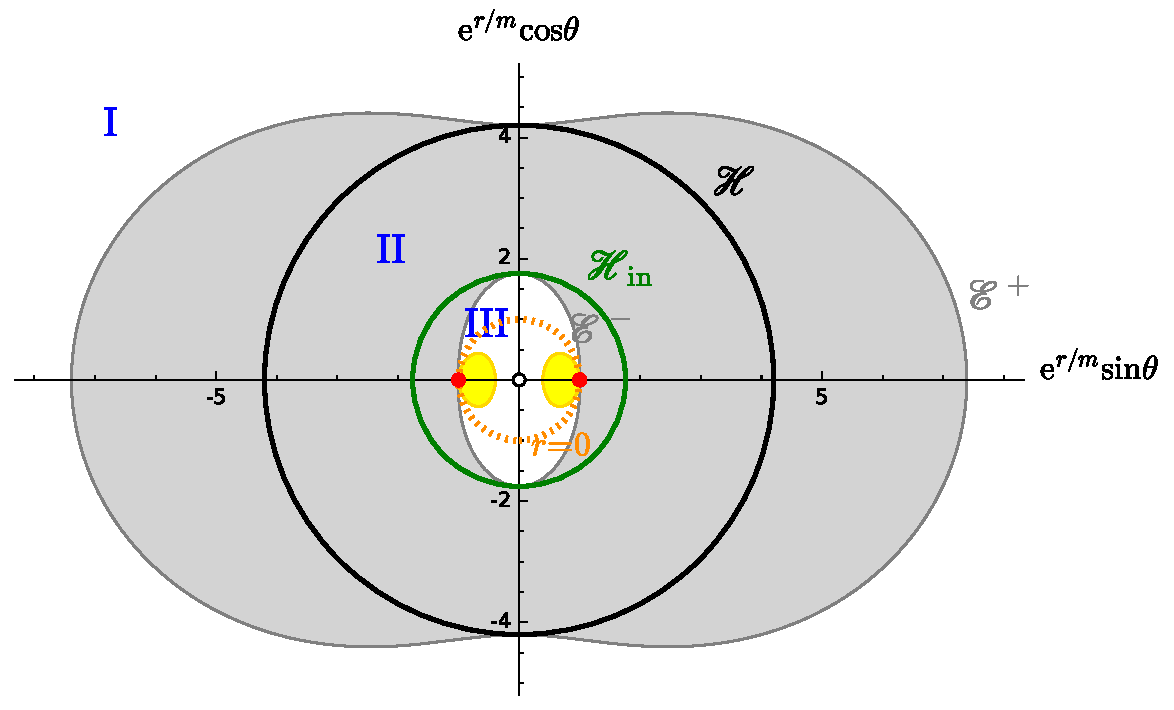
\includegraphics[width=0.8\textwidth]{ker_ergo_a90.pdf}}
\caption[]{\label{f:ker:ergo_a90} \footnotesize
Meridional view of a section $t=\mathrm{const}$ of Kerr spacetime with $a/m=0.90$ in
O'Neill exponential coordinates $x = \mathrm{e}^{r/m}\sin\th$ and $z = \mathrm{e}^{r/m}\sin\th$ (cf. Fig.~\ref{f:ker:spher_view}).
The right (resp. left) half of the figure corresponds to $\ph=0$ (resp. $\ph=\pi$).
The Roman numbers I, II, III denote the components $\M_{\rm I}$, $\M_{\rm II}$ and
$\M_{\rm III}$ of the manifold $\M_{\rm BL}$. The dotted orange circle marks the location
of $r=0$, while the small black circle at the center of the figure corresponds to
$r\rightarrow -\infty$. The two red dots marks the curvature singularity $\mathscr{R}$.
The ergoregion (cf. Sec.~\ref{s:ker:ergoregion}) is shown in grey, while the
yellow part is Carter time machine (cf. Sec.~\ref{s:ker:time_machine}).
}
\end{figure}

\begin{figure}
\centerline{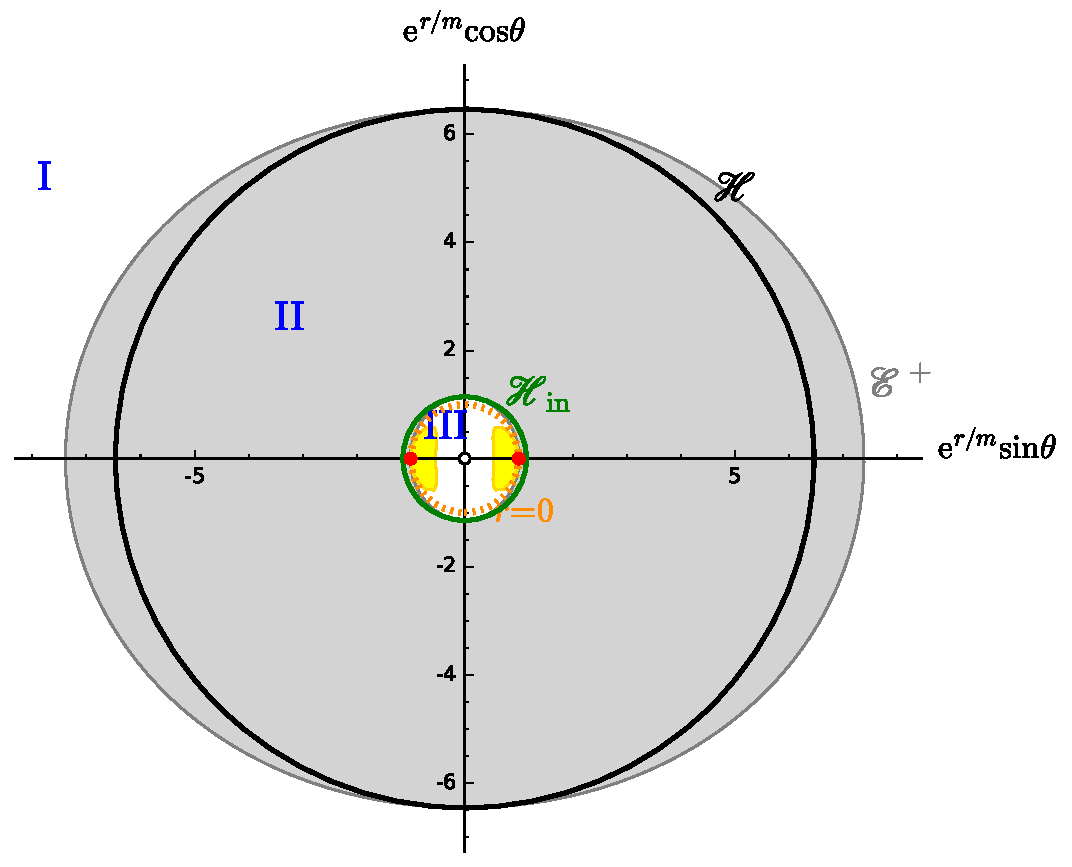
\includegraphics[width=0.6\textwidth]{ker_ergo_a50.pdf}}
\caption[]{\label{f:ker:ergo_a50} \footnotesize
Same as Fig.~\ref{f:ker:ergo_a90} but for $a/m=0.50$.
}
\end{figure}

\begin{figure}
\centerline{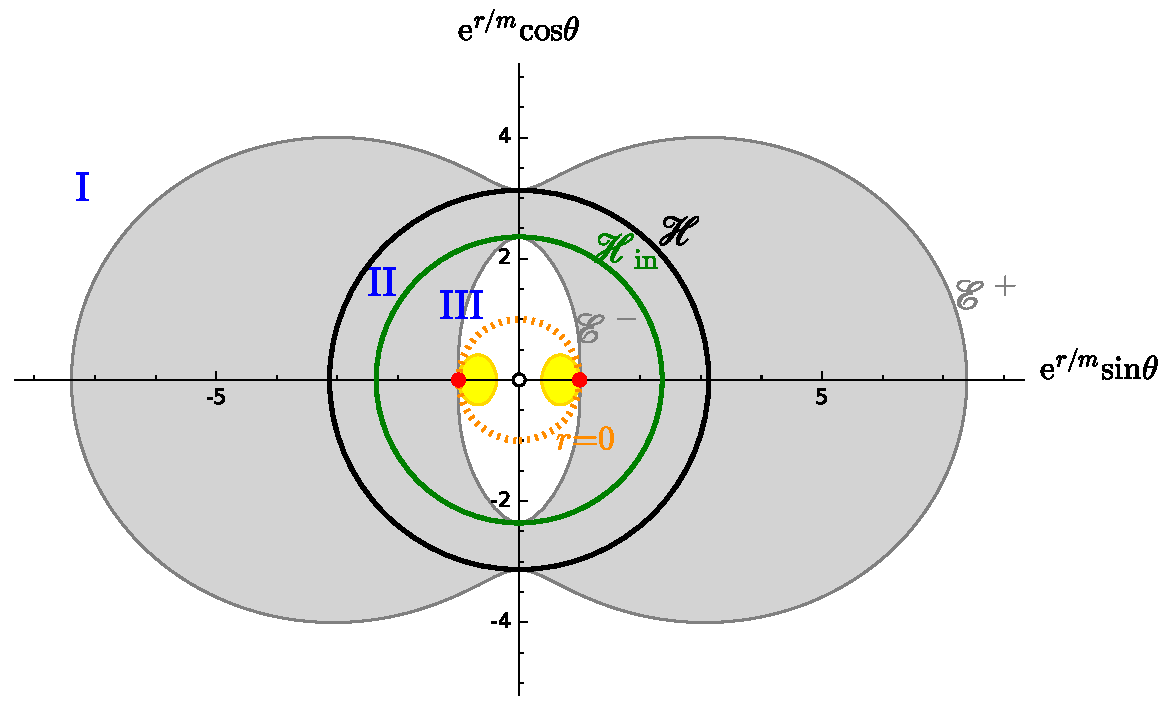
\includegraphics[width=0.8\textwidth]{ker_ergo_a99.pdf}}
\caption[]{\label{f:ker:ergo_a99} \footnotesize
Same as Fig.~\ref{f:ker:ergo_a90} but for $a/m=0.99$.
}
\end{figure}

Given the definition of $\M_{\rm I}$, $\M_{\rm II}$ and $\M_{\rm III}$, we conclude that
\begin{itemize}
\item $\w{\xi}$ is timelike in the region of $\M_{\rm I}$ defined by $r>r_{\E^+}(\theta)$
and in the region of $\M_{\rm III}$ defined by $r<r_{\E^-}(\theta)$;
\item $\w{\xi}$ is null on the hypersurface $\E^+$ of $\M_{\rm I}$ defined by
$r=r_{\E^+}(\theta)$
and on the hypersurface $\E^-$ of $\M_{\rm III}$ defined by $r=r_{\E^-}(\theta)$;
\item $\w{\xi}$ is spacelike in all $\M_{\rm II}$ and in the region
$\mathscr{G}^+$ of $\M_{\rm I}$
defined by $r<r_{\E^+}(\theta)$, as well as
in the region $\mathscr{G}^-$ of $\M_{\rm III}$ defined by $r>r_{\E^-}(\theta)$.
\end{itemize}
According to the nomenclature introduced in Sec.~\ref{s:sta:strong_rigidity},
one calls $\E^+$ (resp. $\E^-$) the
\defin{outer ergosphere}\index{outer!ergosphere}\index{ergosphere!outer --}
(resp. \defin{inner ergosphere}\index{inner!ergosphere}\index{ergosphere!inner --})
and $\mathscr{G}^+$ (resp. $\mathscr{G}^-$) the
\defin{outer ergoregion}\index{outer!ergoregion}\index{ergoregion!outer --}
(resp. \defin{inner ergoregion}\index{inner!ergoregion}\index{ergoregion!inner --}).
The part of $\M_{\rm BL}$ where $\w{\xi}$ is spacelike, i.e.
$\mathscr{G} = \mathscr{G}^+ \cup \M_{\rm II} \cup \mathscr{G}^-$,
is called the \defin{ergoregion}\index{ergoregion!of Kerr spacetime}.
It is depicted in Figs.~\ref{f:ker:ergo_a90}-\ref{f:ker:ergo_a99}.
\begin{remark}
Sometimes the word \defin{ergosurface}\index{ergosurface} is used instead of
\emph{ergosphere}.
\end{remark}


\subsection{Carter time machine} \label{s:ker:time_machine}

Let us now focus on the second Killing vector, $\w{\eta}$.
From (\ref{e:ker:metric_BL}) and (\ref{e:ker:def_rho2}), we have
\[
    \w{\eta}\cdot\w{\eta} = g_{\ph\ph} = \left( r^2 + a^2 + \frac{2 a^2 m r \sin^2\th}{r^2 + a^2\cos^2\th} \right) \sin^2\th .
\]
Hence
\[
    \w{\eta}\ \mbox{spacelike} \iff
        (r^2 + a^2)(r^2 + a^2\cos^2\th) + 2 a^2 m r \sin^2\th > 0 .
\]
For $\theta\rightarrow 0$ or $\theta\rightarrow\pi$, the left-hand side of the above equality
is always positive, but for $\theta=\pi/2$ and $r$ negative with $|r|$
small enough so that $2 a^2 m |r| > r^2(r^2 + a^2)$, it is negative. This feature
is apparent on Fig.~\ref{f:ker:sign_gpp}: for $\theta$ close to $\pi/2$,
there is a region $\mathscr{T}$ defined by $r_{\mathscr{T}}(\theta) < r < 0$ for some
negative function $r_{\mathscr{T}}(\theta)$, such that $g_{\ph\ph}<0$.
Since $\mathscr{T}$ corresponds to negative values of $r$, we have
$\mathscr{T}\subset \M_{\rm III}$.
Hence we conclude:
\begin{itemize}
\item $\w{\eta}$ is spacelike in all $\M_{\rm I}$ and $\M_{\rm II}$, as well
as outside the region $\mathscr{T}$ in $\M_{\rm III}$;
\item $\w{\eta}$ is timelike in the subset $\mathscr{T}$ of $\M_{\rm III}$;
\item $\w{\eta}$ is null at the boundary of $\mathscr{T}$.
\end{itemize}
The region $\mathscr{T}$ is called
\defin{Carter time machine}\index{Carter!time machine}\index{time!machine (Carter)}.
This name stems from the fact that thanks to $\mathscr{T}$, there is
a future-directed timelike curve connecting any two points of $\M_{\rm III}$
(see e.g. Proposition~2.4.7 of O'Neill's textbook \cite{ONeil95} for a
demonstration, or Carter's original article \cite{Carte68}).
The region $\mathscr{T}$ is depicted in yellow in the meridional
diagrams of
Figs.~\ref{f:ker:ergo_a90}-\ref{f:ker:ergo_a99}.
\begin{figure}
\centerline{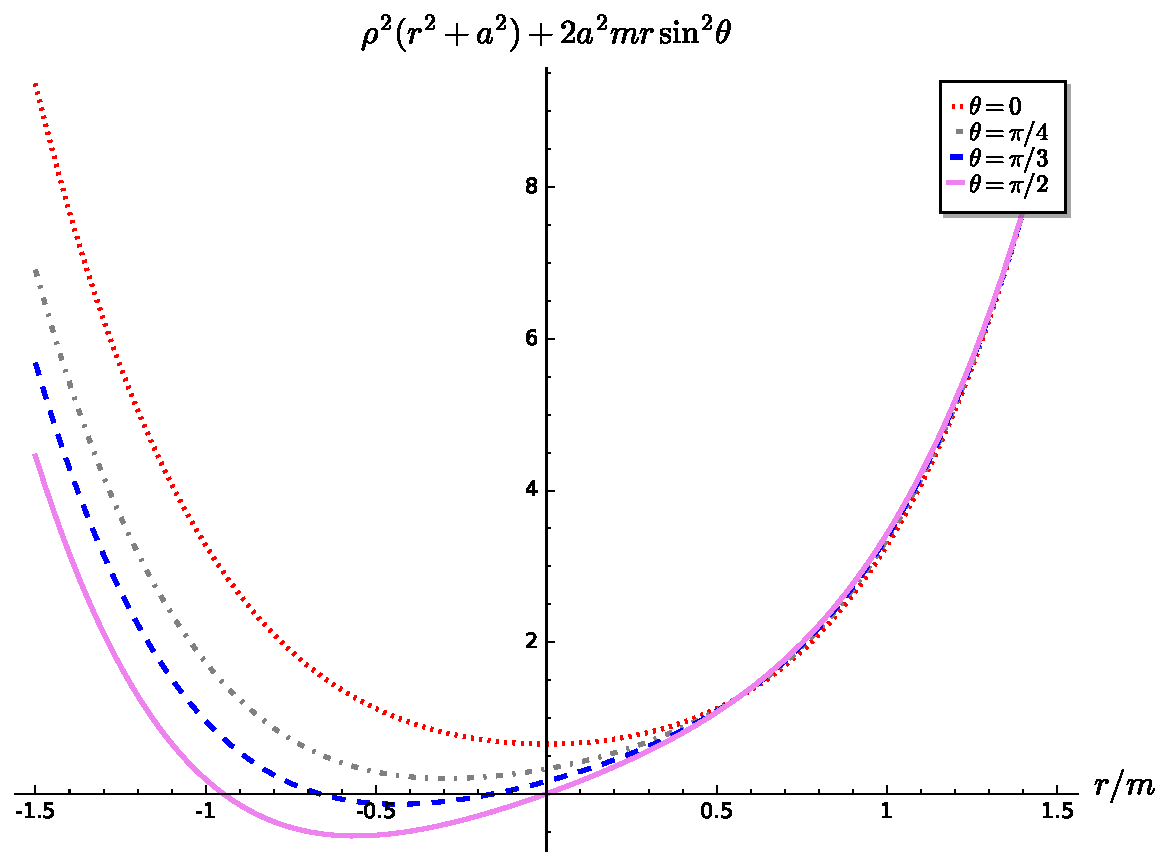
\includegraphics[width=0.7\textwidth]{ker_sign_gpp.pdf}}
\caption[]{\label{f:ker:sign_gpp} \footnotesize
Graph of the function giving the sign of $g_{\ph\ph}$ for $a=0.9m$
and various values of $\theta$.}
\end{figure}


\subsection{Singularities}

The components $g_{\alpha\beta}$ of the Kerr metric as given by  (\ref{e:ker:metric_BL})
are diverging at various locations:
\begin{itemize}
\item when $\rho^2\rightarrow 0$, which, given (\ref{e:ker:def_rho2})
and assuming $a\not=0$, is equivalent to approaching
the cylinder $\ring$ defined by (\ref{e:ker:def_ring});
\item when $\Delta\rightarrow 0$, which, given (\ref{e:ker:def_Delta}), is equivalent to either $r\rightarrow r_-$
or $r\rightarrow r_+$; the first case corresponds to the boundary (within $\R^2\times\SS^2$)
between $\M_{\rm II}$ and $\M_{\rm III}$ and the second case to the boundary
between $\M_{\rm I}$ and $\M_{\rm II}$.
\end{itemize}
The divergence when $\rho^2\rightarrow 0$ corresponds to a
\emph{curvature singularity}\index{curvature!singularity}\index{singularity!curvature --}.
Indeed the Kretschmann scalar of Kerr metric is (cf.
Eq.~(\ref{e:sch:def_Kretschmann}) and Sec.~\ref{s:sam:Kerr_solution} for the computation)
\be
    K := R_{\mu\nu\rho\sigma} R^{\mu\nu\rho\sigma}
     = 48 \frac{m^2}{\rho^{12}} \left( r^6 - 15 r^4 a^2\cos^2\th + 15 r^2 a^4 \cos^4\th - a^6\cos^6\th \right) .
\ee
The value for $\theta=\pi/2$ is thus $K = 48 m^2 / r^6$, which clearly diverges
for $r\rightarrow 0$ (i.e. $\rho^2\rightarrow 0$).
Hence $\ring$ is called the
\defin{ring singularity}\index{ring!singularity}\index{singularity!ring --}
of Kerr spacetime, the word \emph{ring} reflecting the fact that $t=\mathrm{const}$
sections of $\ring$ are circles [cf. Eq.~(\ref{e:ker:ring_R_S1})].

On the contrary, we shall see in the next section that the divergence
of the metric components when $\Delta\rightarrow 0$ corresponds to
a mere
\emph{coordinate singularity}\index{coordinate!singularity}\index{singularity!coordinate --},
i.e. to a pathology of Boyer-Lindquist coordinates, which can be cured by switching to
other coordinates.

%%%%%%%%%%%%%%%%%%%%%%%%%%%%%%%%%%%%%%%%%%%%%%%%%%%%%%%%%%%%%%%%%%%%%%%%

\section{Kerr coordinates and extension of the spacetime manifold}

\subsection{Kerr coordinates} \label{s:ker:Kerr_coord}

The \defin{Kerr coordinates}\index{Kerr!coordinates} are coordinates
$\hat{x}^\alpha = (v,r,\th,\tph)$ defined on $\R^2\times\SS^2$ and related to the Boyer-Lindquist coordinates
$x^\alpha = (t,r,\th,\ph)$ introduced in Sec.~\ref{s:ker:expr_BL} by
\begin{subequations}
\label{e:ker:Kerr_coord}
\begin{align}
& \encadre{\D v = \D t + \frac{r^2+a^2}{\Delta} \, \D r} \label{e:ker:Kerr_coord_v}\\
& \encadre{\D \tph = \D \ph + \frac{a}{\Delta}\, \D r} . \label{e:ker:Kerr_coord_tph}
\end{align}
\end{subequations}
If $a=0$, we note that Kerr coordinates are nothing but the null
ingoing Eddington-Finkelstein
coordinates on Schwarzschild spacetime (cf. Sec.~\ref{s:sch:EF_coord} and compare
(\ref{e:ker:Kerr_coord_v}) with (\ref{e:sch:dt_dv_NIEF})).

Given that $\Delta = (r-r_-)(r-r_+) = r^2+a^2 - 2mr$ [Eq.~(\ref{e:ker:def_Delta})], we have
the identities
\[
    \frac{r^2+a^2}{\Delta} = 1 + \frac{2m}{r_+-r_-} \left( \frac{r_+}{r-r_+}
        - \frac{r_-}{r-r_-} \right) \quad\mbox{and}\quad
     \frac{a}{\Delta} = \frac{a}{r_+-r_-} \left( \frac{1}{r-r_+}
        - \frac{1}{r-r_-} \right) ,
\]
with $r_+-r_- = 2\sqrt{m^2-a^2}$,
so that Eqs.~(\ref{e:ker:Kerr_coord}) can be readily integrated to
\begin{subequations}
\label{e:ker:Kerr_coord_int}
\begin{align}
& \encadre{v = t + r + \frac{m}{\sqrt{m^2-a^2}} \left(
    r_+ \ln\left| \frac{r-r_+}{2m} \right|
    - r_- \ln\left| \frac{r-r_-}{2m} \right| \right) }\label{e:ker:Kerr_coord_v_int}\\
& \encadre{ \tph = \ph + \frac{a}{2\sqrt{m^2-a^2}}\, \ln \left|
    \frac{r-r_+}{r-r_-} \right| } , \label{e:ker:Kerr_coord_tph_int}
\end{align}
\end{subequations}
up to some additive constant.
When $a\rightarrow 0$, we have $r_+\rightarrow 2m$ and $r_-\rightarrow 0$
and by comparing Eq.~(\ref{e:ker:Kerr_coord_v_int}) with Eq.~(\ref{e:sch:v_t_r}), we recover the fact
that the Kerr coordinates reduces to the ingoing Eddington-Finkelstein
ones in this limit.

The components $\hat{g}_{\alpha\beta}$
of the metric tensor $\w{g}$ with respect to the Kerr coordinates
are computed from those with respect to the Boyer-Lindquist ones, as given
by Eq.~(\ref{e:ker:metric_BL}). One gets (cf. Appendix~\ref{s:sam} or
Eq.~(5.31) of Ref.~\cite{HawkiE73}, or Lemma~2.5.2 of \cite{ONeil95}):
\be \label{e:ker:metric_Kerr_coord}
    \begin{array}{ll}
    \hat{g}_{\mu\nu}\,  \D \hat{x}^\mu \D \hat{x}^\nu  = &
    \displaystyle - \left( 1 - \frac{2m r}{\rho^2} \right) \, \D v^2
    + 2 \D v\, \D r
    - \frac{4 a m  r \sin^2\th}{\rho^2} \,  \D v\, \D\tph \\[2ex]
    & - 2 a \sin^2\th \, \D r\, \D \tph  \displaystyle + \rho^2 \D \th^2
    + \left( r^2 + a^2 + \frac{2 a^2 m r \sin^2\th}{\rho^2} \right)
    \sin^2\th \, \D \tph^2 .
    \end{array}
\ee
We note that these metric components do not have any divergence when
$\Delta\rightarrow 0$, contrary to the Boyer-Lindquist ones. Hence, we may extend
the Kerr metric to the points of $\R^2\times\SS^2$ where $\Delta=0$, i.e.
to the hypersurfaces (cf. Fig.~\ref{f:ker:spher_view})
\be
    \Hor := \left\{ p \in \R^2\times\SS^2,\quad r(p) = r_+ \right\}
\ee
and
\be
    \Hor_{\rm in} := \left\{ p \in \R^2\times\SS^2,\quad r(p) = r_- \right\} .
\ee
The hypersurface $\Hor$ is actually the interface between the regions $\M_{\rm I}$
and $\M_{\rm II}$, while $\Hor_{\rm in}$ is the interface between $\M_{\rm II}$
and $\M_{\rm III}$ (cf. Eq.~(\ref{e:ker:M_I_III_r}) and Fig.~\ref{f:ker:ergo_a90}).
We thus consider
\be \label{e:ker:def_M_Kerr_spacetime}
   \encadre{ \M := \M_{\rm BL} \cup \Hor \cup \Hor_{\rm in} = \R^2\times\SS^2 \setminus \ring }
\ee
as the spacetime manifold. In order for $\w{g}$ defined by (\ref{e:ker:metric_Kerr_coord})
to be a well defined metric on $\M$, it does not suffice that the components
$\hat{g}_{\alpha\beta}$ do not diverge at $\Hor$ and $\Hor_{\rm in}$: one shall
check as well that the bilinear form $\w{g}$ is non-degenerate there.
This is easily proven by considering the determinant of the metric components,
which turns out to have a simple form (cf. Sec.~\ref{s:sam:Kerr_Kerr_coord}):
\be
    \det (\hat{g}_{\alpha\beta}) = -\rho^4 \sin^2\th .
\ee
Except at $\th=0$ and $\th=\pi$ (the usual singularity of spherical coordinates),
we have $\det (\hat{g}_{\alpha\beta}) \not= 0$ everywhere on $\M$, since
$\rho$ vanishes only on $\ring$, which is excluded from $\M$.
Hence we conclude that $\w{g}$ is not degenerate on $\M$ and thus
$(\M,\w{g})$ is a well behaved spacetime --- our \defin{Kerr spacetime}\index{Kerr!spacetime}
from now on. We note that, contrary to $\M_{\rm BL}$, $\M$ is a connected manifold.

We deduce from (\ref{e:ker:Kerr_coord}) that the Kerr coordinate frame
is related to the Boyer-Lindquist coordinate frame by
\begin{subequations}
\label{e:ker:frame_Kerr_BL}
\begin{align}
    & \wpar_v = \wpar_t \\
    & \wpar_{\hat{r}} = \wpar_r - \frac{a^2+r^2}{\Delta} \wpar_t
                        - \frac{a}{\Delta} \wpar_\ph \label{e:ker:frame_Kerr_BL_r}\\
    & \wpar_\th = \wpar_\th \\
    & \wpar_{\tph} = \wpar_\ph .
\end{align}
\end{subequations}
Note that we are using the notation $\wpar_{\hat{r}}$ for the $\partial/\partial r$
vector of the Kerr coordinates $\hat{x}^\alpha = (v,r,\th,\tph)$, to distinguish
it from the $\partial/\partial r$ vector of the Boyer-Lindquist coordinates.
We read on (\ref{e:ker:metric_Kerr_coord}) that $\hat{g}_{rr} = 0$, which
implies that $\wpar_{\hat{r}}$ is a global null vector field on $\M$.
We may use it to set the time orientation of $(\M,\w{g})$ by demanding that
\be \label{e:ker:def_k_hat_r}
    \w{k} := - \wpar_{\hat{r}}
\ee
is a future-directed null vector field in all $\M$. The minus sign
in the above definition, along with Eq.~(\ref{e:ker:frame_Kerr_BL_r}),
ensures that
\[
    \w{k} \sim \wpar_t -  \wpar_r  \quad\mbox{when}\
            r \rightarrow +\infty ,
\]
which shows that the time orientation set by $\w{k}$ agrees asymptotically
with that of $\wpar_t$.


The field lines
of $\w{k}$ are future-directed null curves,
which may be qualified of \emph{ingoing} since, by definition, $-\wpar_{\hat{r}}$ points towards
decreasing values of $r$. Note that, by the very definition of $\wpar_{\hat{r}}$,
the values of the coordinates $(v,\th,\tph)$ are fixed along each of these
null curves. We therefore denote them by $\Li^{\rm in}_{(v,\th,\tph)}$.
We shall see in Sec.~\ref{s:ker:principal_geod} that $\Li^{\rm in}_{(v,\th,\tph)}$ is actually a null geodesic.


\begin{hist}
Kerr coordinates are actually those in which R.P.~Kerr originally presented his
solution \cite{Kerr63}. Actually, he used $-\tph$ instead of $\tph$; hence
the correspondance between our notations and those of Kerr's article \cite{Kerr63}
is $v\leftrightarrow u$ and $\tph\leftrightarrow -\phi$.
\end{hist}

\subsection{3+1 Kerr coordinates}

As in Sec.~\ref{s:sch:EF_coord},
we shall move from the null coordinate $v$ to a (asymptotically)
timelike one by setting
\be \label{e:ker:def_t_tilde}
    \encadre{\ti = v - r} \iff \encadre{v = \ti + r}
\ee
so that $v$ appears as the advanced time $\ti+r$ (compare with Eq.~(\ref{e:sch:ti_v_r})). We thus consider
the coordinates
\be
    (\tilde{x}^\alpha) = (\ti, r, \th,\tph) ,
\ee
which we call the
\defin{3+1 Kerr coordinates}\index{3+1!Kerr coordinates}\index{Kerr!coordinates!3+1 --}.
It is worth to relate them to the Boyer-Lindquist coordinates
$(t,r,\th,\ph)$. This is easily achieved
by combining (\ref{e:ker:Kerr_coord}) with $\D\ti = \D v - \D r$:
\begin{subequations}
\label{e:ker:Kerr_3p1_BL}
\begin{align}
& \encadre{\D \ti = \D t + \frac{2m r}{\Delta} \, \D r} \\
& \encadre{\D \tph = \D \ph + \frac{a}{\Delta}\, \D r} .
\end{align}
\end{subequations}
The integrated version is deduced obtained by substituting (\ref{e:ker:def_t_tilde}) in
Eq.~(\ref{e:ker:Kerr_coord_int}):
\begin{subequations}
\begin{align}
& \encadre{\ti = t  + \frac{m}{\sqrt{m^2-a^2}} \left(
    r_+ \ln\left| \frac{r-r_+}{2m} \right|
    - r_- \ln\left| \frac{r-r_-}{2m} \right| \right) }\\
& \encadre{ \tph = \ph + \frac{a}{2\sqrt{m^2-a^2}}\, \ln \left|
    \frac{r-r_+}{r-r_-} \right| } .
\end{align}
\end{subequations}


\begin{hist}
In the historical article \cite{Kerr63}, R.P.~Kerr introduced $\ti$ by exactly
the same transformation as (\ref{e:ker:def_t_tilde}) ($\ti$ is denoted $t$
in \cite{Kerr63}), but along with Cartesian-type coordinates $(x,y,z)$
deduced from $(r,\th,\tph)$ by spheroidal transformations, to form the 3+1
coordinate system $(\ti,x,y,z)$, which is today known as
\defin{Kerr-Schild coordinates}\index{Kerr-Schild coordinates} (despite
they have been introduced first in Kerr's article \cite{Kerr63} (1963) and not
in the article by Kerr and Schild \cite{KerrS65} (1965)). Accordingly,
our ``3+1 Kerr coordinates'' are a mix of the original Kerr coordinates
$(v,r,\th,\tph)$ (cf. the previous historical note)
and the Kerr-Schild coordinates $(\ti,x,y,z)$.
\end{hist}

Since the transform (\ref{e:ker:def_t_tilde}) leads to $\D v = \D\ti + \D r$,
the metric components $\tilde{g}_{\alpha\beta}$ with respect to the
3+1 coordinates $(\ti,r,\th,\tph)$ are easily deduced from
(\ref{e:ker:metric_Kerr_coord}):
\be \label{e:ker:metric_Kerr_3p1}
    \encadre{
    \begin{array}{ll}
    \tilde{g}_{\mu\nu}\,  \D \tilde{x}^\mu \D \tilde{x}^\nu  = &
    \displaystyle - \left( 1 - \frac{2m r}{\rho^2} \right)  \D \ti^2
    + \frac{4m r}{\rho^2} \D\ti\, \D r
    - \frac{4 a m  r \sin^2\th}{\rho^2} \,  \D \ti\, \D\tph \\[2ex]
    &\displaystyle  + \left( 1 + \frac{2m r}{\rho^2} \right) \D r^2
     - 2 a \left( 1 + \frac{2m r}{\rho^2} \right) \sin^2\th \, \D r\, \D \tph \\[2ex]
    & \displaystyle + \rho^2 \D \th^2
    + \left( r^2 + a^2 + \frac{2 a^2 m r \sin^2\th}{\rho^2} \right)
    \sin^2\th \, \D \tph^2 .
    \end{array}
    }
\ee
As a check, we notice the agreement with Eq.~(D.4) of Ref.~\cite{GourgJ06}.

Since we kept $r$, $\th$ and $\tph$ and simply changed
$v$ to $\ti$ via (\ref{e:ker:def_t_tilde}) when moving from the Kerr
coordinates to the 3+1 Kerr coordinates, we easily get the relation
between the two coordinate frames:
\begin{subequations}
\label{e:ker:frame_Kerr3p1_Kerr}
\begin{align}
    & \wpar_\ti = \wpar_v \\
    & \wpar_{\tilde r} = \wpar_v + \wpar_{\hat{r}} \\
    & \wpar_\th = \wpar_\th \\
    & \wpar_\tph = \wpar_\ph .
\end{align}
\end{subequations}
Note that we have denoted by $\wpar_{\tilde r}$ the second vector of the
coordinate frame associated to the 3+1 Kerr coordinates
$(\tilde{x}^\alpha) = (\ti, r, \th,\tph)$, in order to distinguish it from
the coordinate vector $\wpar_{\hat r}$ of the Kerr coordinates
$(\hat{x}^\alpha) = (v, r, \th,\tph)$, as well as from the coordinate vector
$\wpar_r$ of the Boyer-Lindquist coordinates
$(x^\alpha) = (t,r,\th,\ph)$.

By combining (\ref{e:ker:frame_Kerr_BL}) and (\ref{e:ker:frame_Kerr3p1_Kerr}),
we get the relation between the 3+1 Kerr coordinate frame and the
Boyer-Lindquist coordinate frame:
\begin{subequations}
\label{e:ker:frame_Kerr3p1_BL}
\begin{align}
    & \wpar_\ti = \wpar_t \label{e:ker:frame_Kerr3p1_BL_t} \\
    & \wpar_{\tilde r} = \wpar_r - \frac{2mr}{\Delta} \wpar_t
                        - \frac{a}{\Delta} \wpar_\ph \\
    & \wpar_\th = \wpar_\th \\
    & \wpar_{\tph} = \wpar_\ph . \label{e:ker:frame_Kerr3p1_BL_ph}
\end{align}
\end{subequations}
We notice on (\ref{e:ker:frame_Kerr3p1_BL_t}) and (\ref{e:ker:frame_Kerr3p1_BL_ph})
that the coordinate frame vectors $\wpar_\ti$ and $\wpar_\tph$
coincide with the Killing vectors $\w{\xi}$ and $\w{\eta}$:
\be \label{e:ker:Killing_vec_3p1}
    \encadre{\wpar_\ti = \w{\xi}} \quad \mbox{and} \quad
    \encadre{\wpar_\tph = \w{\eta}} .
\ee
That $\wpar_\ti$ and $\wpar_\tph$ are Killing vectors is not surprising since
the metric components (\ref{e:ker:metric_Kerr_3p1}) do not depend on $\ti$
nor on $\tph$.

The determinant of the metric components (\ref{e:ker:metric_Kerr_3p1}) takes
a very simple form (cf. Sec.~\ref{s:sam:Kerr_Kerr_coord} for the computation):
\be \label{e:ker:det_g_3p1}
    \det\left( \tilde{g}_{\alpha\beta} \right) = - \rho^4\sin^2\th .
\ee
The inverse metric takes also a rather simple form in terms of the 3+1
Kerr coordinates (cf. Sec.~\ref{s:sam:Kerr_Kerr_coord} for the computation):
\be \label{e:ker:inv_met_3p1}
    \tilde{g}^{\alpha\beta} = \left(
    \begin{array}{cccc}
    - \left( 1 + \frac{2m r}{\rho^2} \right) & \frac{2m r}{\rho^2} & 0 & 0 \\[1ex]
    \frac{2m r}{\rho^2} & \frac{\Delta}{\rho^2} & 0 & \frac{a}{\rho^2} \\[1ex]
    0 & 0 &\frac{1}{\rho^2} & 0 \\[1ex]
    0 & \frac{a}{\rho^2} & 0 & \frac{1}{\rho^2\sin^2\th}
    \end{array}
    \right) .
\ee

Comparing (\ref{e:ker:frame_Kerr3p1_BL}) with (\ref{e:ker:metric_BL}), we
note that the metric components in 3+1 Kerr coordinates are slightly more
complicated than those in Boyer-Lindquist coordinates, for they contain
extra non-diagonal terms: ${\tilde g}_{\ti r}$ and ${\tilde g}_{r \tph}$. However
the determinant (\ref{e:ker:det_g_3p1})
and the inverse metric (\ref{e:ker:inv_met_3p1}) are pretty simple. Morever
the 3+1 Kerr coordinates are as well adapted to the spacetime symmetries
as the Boyer-Lindquist ones, as (\ref{e:ker:Killing_vec_3p1}) shows, and
they have the great advantage to be regular on the boundary hypersurfaces
$\Hor$ and $\Hor_{\rm in}$, contrary to the Boyer-Lindquist ones.
The last feature is all the more important since
$\Hor$ is the future event horizon of Kerr spacetime,
as we are going to see.
Therefore, we shall continue our study of Kerr spacetime, and especially the
black hole aspect, by means of the 3+1 Kerr coordinates.

\begin{remark} \label{r:ker:Kerr_slicing}
Despite we called them ``3+1 Kerr coordinates'', the coordinates
$(\ti,r,\th,\tph)$ are not related everywhere to a 3+1 slicing of
spacetime. By 3+1 slicing\index{3+1 slicing}, it is indeed meant a foliation of $\M$
by spacelike hypersurfaces (see e.g. \cite{Gourg12}). Now, the hypersurfaces
$\ti = \mathrm{const}$ are spacelike iff their normal $\vec{\nabla} \ti$ is timelike, which
is equivalent to $\w{g}(\vec{\nabla} \ti, \vec{\nabla} \ti) < 0$, with
\[
    \w{g}(\vec{\nabla} \ti, \vec{\nabla} \ti) = g_{\mu\nu} \, \nabla^\mu \ti \nabla^\nu \ti
    = g^{\mu\nu}\,  \partial_\mu \ti \, \partial_\nu \ti = g^{\ti\ti} .
\]
Given the value of $g^{\ti\ti}$ read on (\ref{e:ker:inv_met_3p1}), the hypersurface
$\ti=\mathrm{const}$ is spacelike iff $\rho^2+2mr > 0$, or equivalently
$r^2 + 2 mr + a^2\cos^2\th > 0$. Now this second-order polynomial is positive everywhere except in the region of $\M_{\rm III}$ defined by
\be \label{e:ker:no_slicing}
    - m - \sqrt{m^2-a^2\cos^2\th} \leq r \leq -m + \sqrt{m^2-a^2\cos^2\th} .
\ee
Note that this region is contained in the part $r\leq 0$  of $\M_{\rm III}$.
We conclude that the coordinates $(\ti,r,\th,\tph)$ define a 3+1 slicing of $\M$
in $\M_{\rm I}$, $\M_{\rm II}$ and in the part of $\M_{\rm III}$ outside the
region defined by (\ref{e:ker:no_slicing}).
\end{remark}

\subsection{Principal null geodesics} \label{s:ker:principal_geod}

We have seen that the Kerr coordinates $(v,r,\th,\tph)$ introduced in
Sec.~\ref{s:ker:Kerr_coord} are such that
the curves $\Li^{\rm in}_{(v,\th,\tph)}$ defined by $(v,\th,\tph)=\mathrm{const}$ are null curves. Their future-directed tangent
vector field is $\w{k} = -\wpar_{\hat{r}}$ [Eq.~(\ref{e:ker:def_k_hat_r})], which
can expressed in terms of 3+1 Kerr
basis via (\ref{e:ker:frame_Kerr3p1_Kerr}):
\be \label{e:ker:k_ti_tr}
    \w{k} = \wpar_\ti - \wpar_{\tilde r} .
\ee
In Sec.~\ref{s:sam:Kerr_Kerr_coord}, it is shown by a direct computation
that
\be \label{e:ker:nab_k_k}
    \wnab_{\w{k}}\, \w{k} = 0.
\ee
It follows that each curve $\Li^{\rm in}_{(v,\th,\tph)}$ is a geodesic
and that the parameter associated $\lambda$ associated with $\w{k}$, is an
affine parameter of this geodesic. We can choose $\lambda=-r$ since
(\ref{e:ker:k_ti_tr}) implies
\[
    k^r = \frac{\D r}{\D\lambda} = - 1 .
\]
The geodesics $\Li^{\rm in}_{(v,\th,\tph)}$
are called the \defin{ingoing principal null geodesics}\index{principal!null geodesic}.
The qualifier \emph{ingoing} stems from the fact that $r$ is decreasing along
$\Li^{\rm in}_{(v,\th,\tph)}$ (in the future direction), which is an
immediate consequence of $\lambda=-r$ being a future-oriented parameter along $\Li^{\rm in}_{(v,\th,\tph)}$.
The qualifier \emph{principal} arises from a relation between $\w{k}$
and the Weyl conformal curvature tensor $\w{C}$ (cf. Sec.~\ref{s:bas:Weyl})
of Kerr spacetime, namely:
\be
    C^\alpha_{\ \, \mu\nu[\beta} k_{\gamma]} k^\mu k^\nu = 0
    \qquad\mbox{and}\qquad
    {}^*C^\alpha_{\ \, \mu\nu[\beta} k_{\gamma]} k^\mu k^\nu = 0 ,
\ee
where  ${}^*\w{C}$ stands for the
\defin{dual of the Weyl tensor}\index{dual!of Weyl tensor}\index{Weyl curvature tensor!dual}:
\be
    {}^*C^\alpha_{\ \, \beta\gamma\delta} := \frac{1}{2} \, C^\alpha_{\ \, \beta\mu\nu}
    \, \epsilon^{\mu\nu}_{\ \ \, \gamma\delta} ,
\ee
$\w{\epsilon}$ being the Levi-Civita tensor (cf. Sec.~\ref{s:bas:Levi-Civita_tensor}).
One says that the vector field $\w{k}$ defines a \emph{doubly degenerate, principal null
direction} of $\w{C}$ (see e.g. Chap.~5 of O'Neill textbook \cite{ONeil95} for
details).

\begin{figure}
\centerline{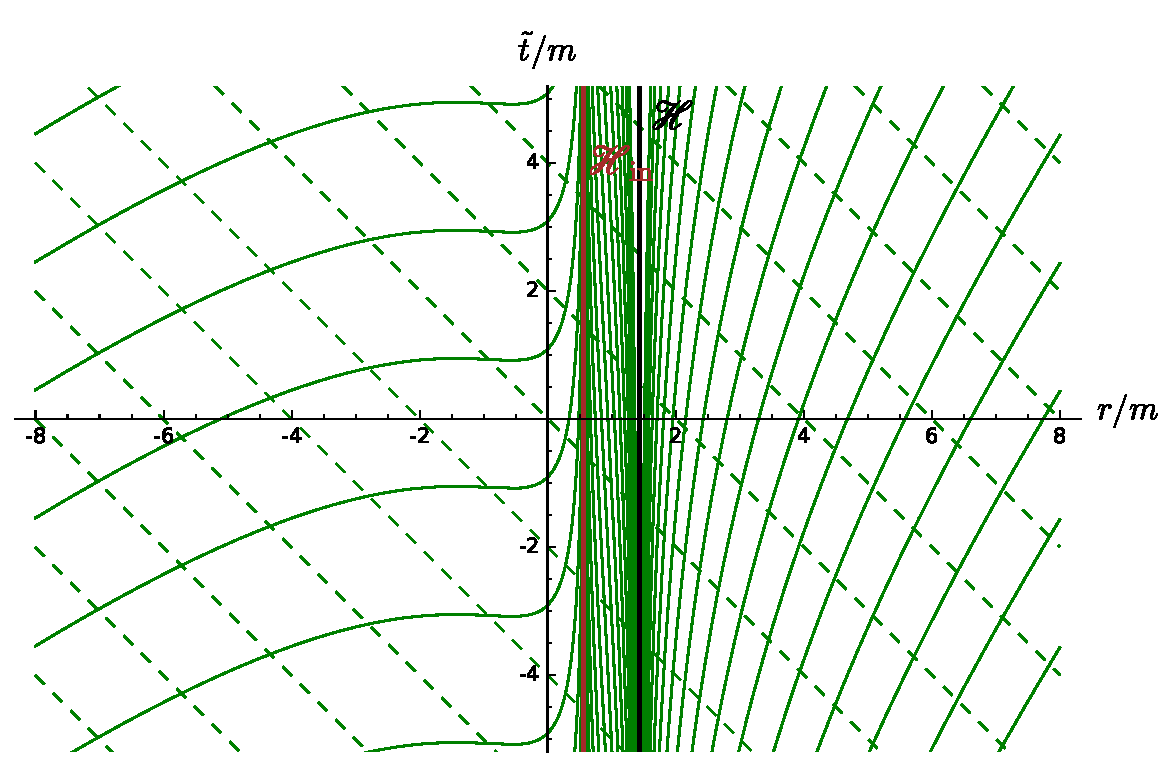
\includegraphics[width=0.9\textwidth]{ker_princ_null_geod_a90.pdf}}
\caption[]{\label{f:ker:princ_null_geod_a90} \footnotesize
Principal null geodesics of Kerr spacetime viewed in terms of the 3+1 Kerr
coordinates $(\ti,r)$ for $a/m=0.9$. The solid (resp. dashed) curves
correspond to outgoing geodesics $\Li^{\rm out}_{(u,\th,\tilde{\tph})}$
(resp. incoming geodesics $\Li^{\rm in}_{(v,\th,\tph)}$), as given by
Eq.~(\ref{e:ker:out_princ_geod}) with $u=\mathrm{const}$
(resp. Eq.~(\ref{e:ker:def_t_tilde}) with $v=\mathrm{const}$). The increment
in $u$ between two depicted outgoing geodesics is $\delta u = 2m$;
similarly, two depicted ingoing geodesics differ in their values of
$v$ by $\delta v = 2m$.
}
\end{figure}

\begin{figure}
\centerline{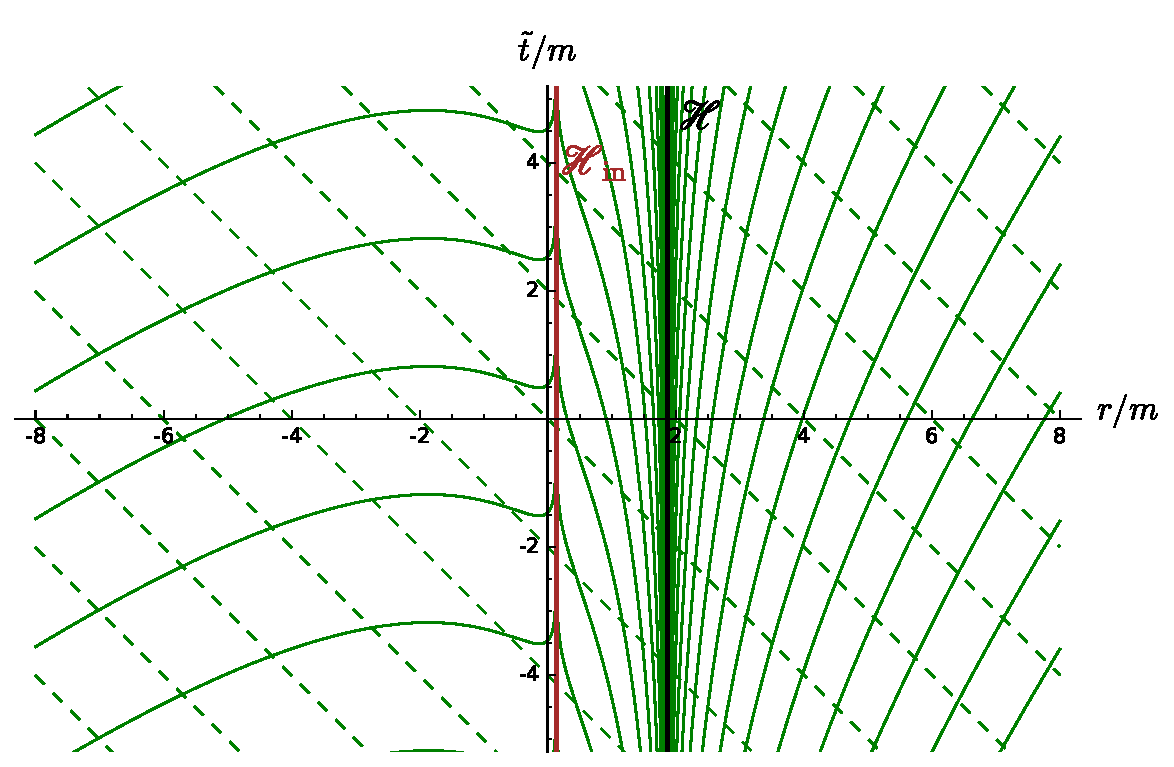
\includegraphics[width=0.9\textwidth]{ker_princ_null_geod_a50.pdf}}
\caption[]{\label{f:ker:princ_null_geod_a50} \footnotesize
Same as Fig.~\ref{f:ker:princ_null_geod_a90}, but for $a/m=0.5$.}
\end{figure}


We note that the ingoing principal null geodesics form a \emph{congruence}: through
each point of $\M$, there is one, and only one, curve $\Li^{\rm in}_{(v,\th,\tph)}$.

One can construct a second congruence of principal null geodesics from
the \emph{outgoing} Kerr coordinates instead of the ingoing ones
considered in Sec.~\ref{s:ker:Kerr_coord}. The \defin{outgoing Kerr coordinates}
$(u,r,\th,\tilde{\tph})$ are defined by relations to Boyer-Lindquist
coordinates that are similar to
(\ref{e:ker:Kerr_coord}), up to a change of sign:
\begin{subequations}
\label{e:ker:out_Kerr_coord}
\begin{align}
& \D u = \D t - \frac{r^2+a^2}{\Delta} \, \D r \\
& \D \tilde{\tph} = \D \ph - \frac{a}{\Delta}\, \D r .
\end{align}
\end{subequations}
The coordinates $(u,r,\th,\tilde{\tph})$ generalize the null
outgoing Eddington-Finkelstein
coordinates introduced in Sec.~\ref{s:sch:BH} to the case $a\not=0$.
Thanks to the symmetry $(t,\ph)\mapsto(-t,-\ph)$ of the Kerr metric (\ref{e:ker:metric_BL}), which turns $(u,\tilde{\tph})$ into $(-v,-\tph)$, it is clear that the curves $\Li^{\rm out}_{(u,\th,\tilde{\tph})}$
defined by $(u,\th,\tilde{\tph})=\mathrm{const}$ constitute a second
congruence of principal null geodesics, called the \defin{outgoing principal null geodesics}\index{principal!null geodesic}. As $-r$ was a affine parameter along
the ingoing principal null geodesics, $r$ is an affine parameter along
the outgoing principal null geodesics,
 except at the locations of $\M$ where $\Delta=0$,
i.e. at $\Hor$ and $\Hor_{\rm in}$ (see below). Another difference
with respect to the ingoing family is that, while $-r$ was always
increasing towards the future along ingoing geodesics,
 $r$ is increasing towards the future
along outgoing principal null geodesics only in regions
$\M_{\rm I}$ and $\M_{\rm III}$; in region $\M_{\rm II}$,
$r$ is decreasing towards the future.

The fact that the Weyl tensor $\w{C}$
admits two, and exactly two, congruences of principal null geodesics
means that the Kerr metric is an \emph{algebraically special} solution of
Einstein equation: it belongs to the so-called \emph{Petrov type D}\index{Petrov type}.

In this chapter, we shall focus on
the expression of the outgoing principal null geodesics in terms of
the 3+1 Kerr coordinates.
Combining (\ref{e:ker:out_Kerr_coord}) with (\ref{e:ker:Kerr_3p1_BL}),
we get
\begin{subequations}
\label{e:ker:out_Kerr_Kerr_3p1}
\begin{align}
& \D u = \D \ti - \frac{r^2 + 2m r + a^2}{\Delta} \, \D r \\
& \D \tilde{\tph} = \D \tph - \frac{2a}{\Delta}\, \D r .
\end{align}
\end{subequations}
These equations can be integrated (cf. the computation leading to Eq.~(\ref{e:ker:Kerr_coord_int})), yielding
\begin{subequations}
\label{e:ker:out_princ_geod}
\begin{align}
& \ti = u + r + \frac{2m}{\sqrt{m^2-a^2}} \left(
    r_+ \ln\left| \frac{r-r_+}{2m} \right|
    - r_- \ln\left| \frac{r-r_-}{2m} \right| \right) \\
&  \tph = \tilde{\tph} + \frac{a}{\sqrt{m^2-a^2}}\, \ln \left|
    \frac{r-r_+}{r-r_-} \right|  ,
\end{align}
\end{subequations}

The outgoing principal null geodesics are depicted, along with the
ingoing ones, are depicted in Figs.~\ref{f:ker:princ_null_geod_a90} and
\ref{f:ker:princ_null_geod_a50}.
Note that in both asymptotically flat regions, $r\rightarrow +\infty$ and
$r\rightarrow -\infty$, the two congruences of geodesics are $\pm 45^\circ$ lines.
Note also that, despite their name, the outgoing geodesics are actually
ingoing in $\M_{\rm II}$ (between $\Hor_{\rm in}$ and $\Hor$), i.e. have $r$ decaying
towards the future.
\begin{remark}
In Fig.~\ref{f:ker:princ_null_geod_a50},
the outgoing geodesics seem to go ``backward in time'' for $-2m \lesssim r \lesssim 0$. This
is an artifact due to the hypersurfaces $\ti = \mathrm{const}$ being not spacelike
there, as discussed in Remark~\ref{r:ker:Kerr_slicing}
p.~\pageref{r:ker:Kerr_slicing}.
Consequently it is possible to move to the future with decaying values
of $\ti$ in this region.
The same effect exists, but is less pronounced, for $a/m=0.9$ (Fig.~\ref{f:ker:princ_null_geod_a90}).
\end{remark}


Along a null geodesic $\Li^{\rm out}_{(u,\th,\tilde{\tph})}$, we have
$\D u = 0$ and $\D\tilde{\tph}=0$, so that (\ref{e:ker:out_Kerr_Kerr_3p1}) yields
\begin{align}
& \frac{\D \ti}{\D r} =   \frac{r^2 + 2m r + a^2}{\Delta}  \nonumber \\
& \frac{\D \tph}{\D r} = \frac{2a}{\Delta} . \nonumber
\end{align}
As claimed above, these equations show that $r$ cannot be considered as
a parameter along $\Li^{\rm out}_{(u,\th,\tilde{\tph})}$ as soon as
$\Delta=0$, i.e. on $\Hor$ and $\Hor_{\rm in}$.
In order to have a parametrization regular everywhere in $\M$, let us introduce
instead of $r$
the parameter $\lambda$ such that
\[
    \frac{\D r}{\D\lambda} = \frac{\Delta}{2(r^2+a^2)} .
\]
The vector $\wl$ tangent to $\Li^{\rm out}_{(u,\th,\tilde{\tph})}$ and associated
to $\lambda$ has then the following components w.r.t. the 3+1 Kerr coordinates:
\begin{align}
& \ell^{\ti} = \frac{\D \ti}{\D\lambda} = \frac{\D \ti}{\D r}\times\frac{\D r}{\D\lambda}
    = \frac{r^2 + 2m r + a^2}{2(r^2+a^2)} = \frac{1}{2} + \frac{m r}{r^2 + a^2} \nonumber \\
& \ell^{r} = \frac{\D r}{\D\lambda} = \frac{\Delta}{2(r^2+a^2)} = \frac{1}{2} - \frac{m r}{r^2 + a^2}\nonumber \\
& \ell^{\th} = \frac{\D \th}{\D\lambda} = 0 \nonumber\\
& \ell^{\tph} = \frac{\D \tph}{\D\lambda} = \frac{\D \tph}{\D r}\times\frac{\D r}{\D\lambda}
    = \frac{a}{r^2+a^2} . \nonumber
\end{align}
In other words, we have
\be \label{e:ker:def_ell_outgoing}
    \wl = \left( \frac{1}{2} + \frac{m r}{r^2 + a^2} \right) \wpar_\ti
        + \left( \frac{1}{2} - \frac{m r}{r^2 + a^2} \right) \wpar_{\tilde r}
        + \frac{a}{r^2+a^2} \, \wpar_\tph .
\ee
It is clear that this vector field is regular everywhere in $\M$.
Given the metric components (\ref{e:ker:metric_Kerr_3p1}), it is easy
to check that $\w{g}(\wl,\wl)=0$, i.e. that $\wl$ is a null vector.
Moreover, an explicit computation (cf. Sec.~\ref{s:sam:Kerr_Kerr_coord}) reveals that
\be \label{e:ker:pregeod_ell}
    \wnab_{\wl}\, \wl = \bar{\kappa} \, \wl ,
\ee
with
\be \label{e:ker:bar_kappa}
    \bar{\kappa} := \frac{m(r^2-a^2)}{(r^2+a^2)^2} .
\ee
This confirms that the null curves $\Li^{\rm out}_{(u,\th,\tilde{\tph})}$ are
geodesics (cf. Sec.~\ref{s:def:geod_gener}). The fact that
$\bar{\kappa}\not=0$ means that
$\lambda$ is not an affine parameter along $\Li^{\rm out}_{(u,\th,\tilde{\tph})}$.

\begin{remark}
The reader may have noticed a certain dissymmetry between the tangent vector
$\w{k}$ of ingoing principal null geodesics, which obeys $\wnab_{\w{k}}\, \w{k} = 0$
[Eq.~(\ref{e:ker:nab_k_k})] and the tangent vector $\wl$ of the outgoing
ones, which obeys $\wnab_{\wl}\, \wl \not= 0$ [Eq.~(\ref{e:ker:pregeod_ell})].
As mentioned above, the last property is related to the fact that the
parameter $\lambda$ associated to $\wl$ is not affine, while the
parameter $-r$ associated to $\w{k}$ is.
The non-affine choice is the price to pay to have a parametrization of the outgoing
family well defined everywhere on $\M$, even where $\Delta=0$. We shall see in
Sec.~?? that in the maximal extension of the Kerr spacetime, there are other regions
where these features of ingoing and outgoing principal null geodesics are reversed,
thereby restauring the symmetry between them.
\end{remark}

%%%%%%%%%%%%%%%%%%%%%%%%%%%%%%%%%%%%%%%%%%%%%%%%%%%%%%%%%%%%%%%%%%%%%%%%%%%%%%%

\section{Event horizon}

\subsection{Killing horizons} \label{s:ker:Killing_hor}

Let us consider the hypersurfaces of $\M$ defined by a fixed value of
the coordinate $r$. $\Hor$ and $\Hor_{\rm in}$ are two particular cases,
corresponding to $r=r_+$ and $r=r_-$ respectively.
The normal 1-form to these hypersurfaces is $\dd r$; the corresponding
gradient vector field is $\vw{\nabla} r$, the components of which are
$\nabla^\alpha r = g^{\alpha\mu} \partial_\mu r = g^{\alpha r}$.
According to (\ref{e:ker:inv_met_3p1}), we have
\be \label{e:ker:nab_r_comp}
    \nabla^\alpha r = \left( \frac{2m r}{\rho^2}, \frac{\Delta}{\rho^2}, 0, \frac{a}{\rho^2}
            \right) .
\ee
It is then quite natural to consider the vector field
\be \label{e:ker:def_normal_hyp_r}
    \w{n} := \rho^2 \vw{\nabla} r
\ee
for the normal to the hypersurfaces $r=\mathrm{const}$. According to (\ref{e:ker:nab_r_comp}),
it has indeed simple components on the 3+1 Kerr frame:
\be \label{e:ker:normal_r}
    \w{n} = 2 m r \, \wpar_\ti + \Delta \, \wpar_{\tilde r} + a \, \wpar_\tph .
\ee
The scalar square of $\w{n}$ is
\[
    \w{n}\cdot\w{n} = \w{g}(\w{n},\w{n}) = n_\mu n^\mu = \rho^2 (\nabla_\mu r) n^\mu
    = \rho^2 n^r .
\]
Hence, in view of (\ref{e:ker:normal_r}),
\be
    \w{n}\cdot\w{n} = \rho^2 \Delta .
\ee
Since $\rho^2>0$ everywhere on $\M$ and $\Delta = (r-r_+)(r-r_-)$ [cf. Eq.~(\ref{e:ker:def_Delta})], we conclude that
\begin{greybox}
\begin{itemize}
\item The hypersurfaces $r=\mathrm{const}$ are timelike in regions $\M_{\rm I}$ and $\M_{\rm III}$;
\item The hypersurfaces $r=\mathrm{const}$ are spacelike in region $\M_{\rm II}$;
\item $\Hor$ (where $r=r_+$) and $\Hor_{\rm in}$ (where $r=r_-$) are null hypersurfaces.
\end{itemize}
\end{greybox}

On $\Hor$ and $\Hor_{\rm in}$, $\Delta=0$, so that
Eqs.~(\ref{e:ker:nab_r_comp})-(\ref{e:ker:def_normal_hyp_r})
yield
\be \label{e:ker:normal_r_Killing}
    \w{n} = 2 m r_{\pm} \, \wpar_\ti + a \, \wpar_\tph = 2 m r_{\pm} \, \w{\xi}
        + a \, \w{\eta} ,
\ee
where we have used (\ref{e:ker:Killing_vec_3p1}) and $r_{\pm}$ stands for
$r_+$ on $\Hor$ and $r_-$ on $\Hor_{\rm in}$.
On $\Hor$, we may rewrite this expression as
\be \label{e:ker:n_rp_chi}
    \w{n} = 2 m r_+ \, \w{\chi} ,
\ee
with
\be \label{e:ker:def_chi}
    \encadre{\w{\chi} := \w{\xi} + \Omega_H \, \w{\eta} }
\ee
and
\be \label{e:ker:def_OmegaH}
    \encadre{\Omega_H := \frac{a}{2 m r_+} = \frac{a}{r_+^2 + a^2}
        = \frac{a}{2m\left( m + \sqrt{m^2-a^2} \right)} }.
\ee
$\Omega_H$ being a constant, the vector field $\w{\chi}$ defined by
(\ref{e:ker:def_chi}) is a Killing vector field. Moreover, (\ref{e:ker:n_rp_chi})
shows that this Killing vector is normal to the null hypersurface $\Hor$.
In view of the definition given in Sec.~\ref{s:neh:def_Killing_hor}, we
conclude that
\begin{greybox}
$\Hor$ is a Killing horizon\index{Killing!horizon}\index{horizon!Killing --}.
\end{greybox}

Similarly, on $\Hor_{\rm in}$, we may rewrite (\ref{e:ker:normal_r_Killing})
as $\w{n} = 2 m r_- \, \w{\chi}_{\rm in}$, with
\be
    \w{\chi}_{\rm in} := \w{\xi} + \Omega_{\rm in} \, \w{\eta}
\ee
and
\be
    \Omega_{\rm in} := \frac{a}{2 m r_-} = \frac{a}{r_-^2 + a^2}
        = \frac{a}{2m\left( m - \sqrt{m^2-a^2} \right)} ,
\ee
thereby arriving at the same conclusion:
\begin{greybox}
$\Hor_{\rm in}$ is a Killing horizon.
\end{greybox}

\subsection{Event horizon}

As a null hypersurface, $\Hor$ is a one-way membrane (cf. Sec.~\ref{s:def:hor_as_null}),
therefore any (massive or null) particle that crossed it from $\M_{\rm I}$ to
$\M_{\rm II}$ can never be back in $\M_{\rm I}$. Let us show that $\Hor$
is actually a black hole event horizon, as defined in Sec.~\ref{s:glo:def_BH}.

We have seen in Sec.~\ref{s:ker:basic_prop} that the asymptotics of region $\M_{\rm I}$
is the same as that of Schwarzschild spacetime. Hence one can perform a conformal
completion of $(\M_{\rm I},\w{g})$ endowed with a future null infinity $\scri^+$
and a past null infinity $\scri^-$ (an explicit construction of $\scri^+$ and
$\scri^-$ for Schwarzschild spacetime has been performed in
Sec.~\ref{s:max:regul_conf_compl}). A conformal diagram representing $\M_{\rm I}$
along with $\scri^+$
and $\scri^-$ is given in Fig.~\ref{f:ker:3blocks_in} below.


Let us show that the causal past of the future null infinity
coincide with $\M_{\rm I}$: $J^{-}(\scri^+)=\M_{\rm I}$.
Since, as stressed above, no future-directed causal curve can move from $\M_{\rm II}$ to $\M_{\rm I}$
and $\scri^+$ is a boundary of $\M_{\rm I}$, we have $\M_{\rm II} \cap J^{-}(\scri^+) = \varnothing$. A fortiori $\M_{\rm III} \cap J^{-}(\scri^+) = \varnothing$.
We have thus $J^{-}(\scri^+)\subset \M_{\rm I}$. To show the equality between the
two sets there remains to show
that any point $p\in \M_{\rm I}$ can emit a signal reaching $\scri^+$.
Let $\Li$ be the null geodesic through $p$ of the outgoing principal null
congruence $\Li^{\rm out}_{(u,\th,\tilde{\tph})}$ introduced in Sec.~\ref{s:ker:principal_geod}, i.e. $\Li$ is the unique geodesic departing
from $p$ with the tangent vector $\wl$ given by
(\ref{e:ker:def_ell_outgoing}). Along $\Li$, one has
\[
   \frac{\D r}{\D\lambda} = \el^r = \frac{1}{2} - \frac{m r}{r^2 + a^2} ,
\]
where $\lambda$ is the parameter associated with $\wl$.
In particular, at $p$, if we denote by $r_0$ is the $r$-coordinate of $p$ in the 3+1 Kerr system,
\[
    \left. \frac{\D r}{\D\lambda} \right| _{p} = \frac{1}{2} - \frac{m r_0}{r_0^2 + a^2} > 0 .
\]
The above inequality simply translates the fact that $r_0 > r_+$ wherever $p$ lies in
$\M_{\rm I}$.
Hence, initially $r$ is increasing along $\Li$ and we get, since $-mr/(r^2+a^2)$ is an
increasing function of $r$,
\[
    \frac{\D r}{\D\lambda} \geq \frac{1}{2} - \frac{m r_0}{r_0^2 + a^2} =: \alpha > 0.
\]
Since $\alpha$ is a constant, we deduce that
\[
    r \geq r_0 + \alpha(\lambda - \lambda_0) ,
\]
where $\lambda_0$ is the value of $\Li$'s parameter at $p$. When $\lambda\rightarrow +\infty$,
we get $r\rightarrow +\infty$, which proves that the null curve $\Li$
reaches $\scri^+$. Hence we conclude:
\begin{greybox}
$\mathscr{B} = \M \setminus \M_{\rm I}$ is the black hole region, the event
horizon of which is $\Hor$.
\end{greybox}
Incidentally, this illustrates Hawking's strong rigidity theorem discussed
in Sec.~\ref{s:sta:strong_rigidity}: the event horizon of Kerr spacetime
is indeed a Killing horizon, as we have shown in Sec.~\ref{s:ker:Killing_hor}.

According to the discussion in Sec.~\ref{s:sta:strong_rigidity}, we may then
call the quantity $\Omega_H$ introduced in
Eqs.~(\ref{e:ker:def_chi})-(\ref{e:ker:def_OmegaH}) the
\defin{black hole rotation velocity}\index{black hole!rotation velocity}\index{rotation!velocity}.


\subsection{Surface gravity} \label{s:ker:surf_grav}

The null vector field $\wl$ defined by Eq.~(\ref{e:ker:def_ell_outgoing}) coincides with the Killing vector $\w{\chi}$ on $\Hor$,
since $m r/(r^2 + a^2) \equalH 1/2$ and $a/(r^2+a^2) \equalH \Omega_H$:
\be
    \wl \equalH \w{\chi} .
\ee
In view of the pre-geodesic equation (\ref{e:ker:pregeod_ell}) satisfied
by $\wl$, we deduce that
\be \label{e:ker:pregeod_chi}
    \encadre{ \wnab_{\w{\chi}}\, \w{\chi} \equalH \kappa \, \w{\chi} },
\ee
with the non-affinity coefficient\index{non-affinity coefficient} given by Eq.~(\ref{e:ker:bar_kappa})
\[
    \kappa = \left. \bar{\kappa} \right| _{r=r_+} = \frac{m(r_+^2-a^2)}{(r_+^2+a^2)^2} .
\]
$r_+$ being a zero of $\Delta$, we have $r_+^2 + a^2 = 2 m r_+$, so that we may
rewrite the above expression in terms of $r_+$ and $a$ only:
\be
    \kappa = \frac{r_+^2 - a^2}{2r_+(r_+^2+a^2)} .
\ee
Substituting (\ref{e:ker:def_r_pm}) for $r_+$, we get an expression involving
the two basic Kerr parameters:
\be \label{e:ker:kappa_m_a}
    \encadre{ \kappa = \frac{\sqrt{m^2 - a^2}}{2m(m + \sqrt{m^2-a^2})} } .
\ee
Given the strict inequality $a<m$ assumed in this chapter [Eq.~(\ref{e:ker:a_lower_m})],
we have $\kappa\not=0$, which, according to the classification introduced in
Sec.~\ref{s:neh:classif_KH}, means that
\begin{greybox}
As long as $a<m$, the event horizon $\Hor$ is a non-degenerate Killing horizon.
\end{greybox}
In Sec.~\ref{s:neh:surface_gravity}, we have seen that the non-affinity coefficient
$\kappa$ can be interpreted as a ``rescaled'' surface gravity. Hence $\kappa$
is called
the \defin{black hole surface gravity}\index{surface!gravity}\index{gravity!surface --}.
The fact that $\kappa$ is a constant (i.e. does not depend on $\th$) is
an illustration of the \emph{zeroth law of black hole mechanics}
established in Sec.~\ref{s:neh:zeroth_law} (cf. in particular
Example~\ref{x:neh:Schw_Kerr_kappa} in that section).
\begin{remark}
As a check, if we let $a\rightarrow 0$ in Eq.~(\ref{e:ker:kappa_m_a}), we get
$\kappa = 1/(4m)$, i.e. we recover the Schwarzschild horizon value computed in
Example~\ref{x:def:Schw_hor3} of Chap.~\ref{s:def} [cf. Eq.~(\ref{e:def:kappa_Schw_hor})].
\end{remark}

%%%%%%%%%%%%%%%%%%%%%%%%%%%%%%%%%%%%%%%%%%%%%%%%%%%%%%%%%%%%%%%%%%%%%%%%%%%%%%%

\section{Global quantities}

\subsection{Mass} \label{s:ker:Komar_mass}

We have seen in Sec.~\ref{s:ker:basic_prop} that when
$r\rightarrow +\infty$, the Kerr metric tends towards the Schwarzschild
metric of parameter $m$ (cf. Eq.~(\ref{e:ker:asympt_metric}));
we conclude that $m$ is nothing but the gravitational mass $M$ (cf. Sec.~??).
However, for any asymptotically flat spacetime endowed with
an (asymptotically) timelike Killing vector $\w{\xi}$, as the Kerr spacetime,
there is a generic definition of the mass, given by an invariant integral:
the \emph{Komar mass}. We are going to see explicitely
that for the Kerr spacetime, the Komar mass coincides with $m$.

Let $(\M, \w{g})$ be an asymptotically flat spacetime endowed with
a Killing vector $\w{\xi}$ which is timelike at least near infinity.
The \defin{Komar mass}\index{Komar mass}\index{mass!Komar --} is
defined as
\be  \label{e:ker:def_Komar_mass}
    \encadre{M := - \frac{1}{8\pi} \int_{\Sp} \star(\dd \uu{\xi}) },
\ee
where
\begin{itemize}
\item $\Sp$ is a closed spacelike 2-surface;
\item $\uu{\xi}$ is the 1-form associated to the Killing vector $\w{\xi}$
by metric duality (cf. Sec.~\ref{s:bas:metric_dual}), i.e. the 1-form
of components $\xi_\alpha = g_{\alpha\mu} \xi^\mu$, $\dd \uu{\xi}$ is
the exterior derivative of $\uu{\xi}$ (cf. Sec.~\ref{s:bas:ext_deriv} and Eqs.~(\ref{e:bas:def_ext_1f}) and (\ref{e:bas:def_ext_1f_nab})):
\be \label{e:ker:duxi_nab}
    (\dd \uu{\xi})_{\alpha\beta} =
        \partial_\alpha \xi_\beta - \partial_\beta \xi_\alpha =
        \nabla_\alpha \xi_\beta - \nabla_\beta \xi_\alpha
\ee
and $\star(\dd \uu{\xi})$ is the
\defin{Hodge dual}\index{Hodge dual}\index{dual!Hodge --} of the 2-form
$\dd \uu{\xi}$, i.e. the 2-form defined by\footnote{See e.g. Sec.~14.5 of
Ref.~\cite{Gourg13} for an introduction to Hodge duality.}
\be \label{e:ker:star_duxi}
    \star(\dd \uu{\xi}) _{\alpha\beta} := \frac{1}{2}
        (\dd \uu{\xi})_{\mu\nu} \, \epsilon^{\mu\nu}_{\ \ \; \alpha\beta} ,
\ee
$\w{\epsilon}$ being the Levi-Civita tensor associated with the metric $\w{g}$
(cf. Sec.~\ref{s:bas:Levi-Civita_tensor}).
\end{itemize}
An important property of the Komar mass is that its value does not depend
on the choice of the 2-surface $\Sp$, as long as the latter is located
in a vacuum region of spacetime and $\w{g}$ fulfills the Einstein equation
(see e.g. Sec.~8.6.1 of Ref.~\cite{Gourg12} for a demonstration).


\begin{remark}
As the integral of a 2-form over a 2-dimensional manifold, formula
(\ref{e:ker:def_Komar_mass}) is well posed.
\end{remark}
Thanks to the Killing equation (\ref{e:neh:Killing_equation}), one may
rewrite Eq.~(\ref{e:ker:duxi_nab}) as
\be \label{e:ker:dxi_Killing}
    (\dd \uu{\xi})_{\alpha\beta} = 2 \nabla_\alpha \xi_\beta .
\ee
Taking into account Eq.~(\ref{e:ker:star_duxi}), the Komar mass formula
(\ref{e:ker:def_Komar_mass}) becomes then
\be \label{e:ker:def_Komar_mass_alt}
    M = - \frac{1}{8\pi} \int_{\Sp}  \nabla^\mu \xi^\nu \, \epsilon_{\mu\nu\alpha\beta} ,
\ee
where $\omega_{\alpha\beta}:=\nabla^\mu \xi^\nu \, \epsilon_{\mu\nu\alpha\beta}$
stands for the 2-form defined by
$\w{\omega}(\w{u},\w{v}) = \nabla^\mu \xi^\nu \, \epsilon_{\mu\nu\rho\sigma} u^\rho v^\sigma$
for any pair of vector fields $(\w{u},\w{v})$.

Instead of integrals of 2-forms \emph{along} the 2-surface $\Sp$, as in (\ref{e:ker:def_Komar_mass})
and (\ref{e:ker:def_Komar_mass_alt}), one may
express the Komar mass as a \emph{flux integral}\index{flux!integral}\index{integral!flux --}, i.e. the integral of a 2-form
contracted with some ``surface element'', which is \emph{normal} to $\Sp$.
More precisely, let us introduce the
\defin{area element bivector}\index{area!element!bivector}\index{bivector!area element --} by
\be
    \D S^{\alpha\beta} := (s^\alpha n^\beta - n^\alpha s^\beta) \sqrt{q}\, \D x^2 \, \D x^3 ,
\ee
where
\begin{itemize}
\item
$\w{s}$ is a unit spacelike vector normal to $\Sp$ and oriented towards the
exterior of $\Sp$, $\w{n}$ is a unit timelike vector normal to $\Sp$ and oriented towards the
future\footnote{The vector $\w{n}$ considered here shall not be confused with
the vector $\w{n}$ introduced in Sec.~\ref{s:ker:Killing_hor}.}, such that, at each point $p\in\Sp$, $(\w{n},\w{s})$ is an orthonormal basis
of the timelike plane $T^\perp_p\Sp$ normal to $\Sp$.
\item $(x^a)=(x^2,x^3)$ is a coordinate system on $\Sp$
\item $q = \det(q_{ab})$ is the determinant w.r.t. $(x^a)$ of the metric
induced on $\Sp$ by the spacetime metric $\w{g}$, so that
$\sqrt{q}\, \D x^2 \, \D x^3$ is the area element on $\Sp$.
\end{itemize}
To reexpress the Komar mass, we shall use the following identity:\\
\textbf{Lemma}: for any 2-form $\w{A}$ defined in the vicinity of $\Sp$, one has
\be \label{e:ker:int_star_A}
    \int_{\Sp} \star \w{A} = \frac{1}{2} \int_{\Sp} A_{\mu\nu} \, \D S^{\mu\nu} .
\ee
\begin{proof}
Using the definition of the Hodge dual, we have
\[
    \int_{\Sp} \star \w{A} =
        \frac{1}{2} \int_{\Sp} A_{\mu\nu} \, \epsilon^{\mu\nu}_{\ \ \; \alpha\beta} =
        \frac{1}{2} \int_{\Sp} A^{\mu\nu} \, \epsilon_{\mu\nu\alpha\beta} =
         \frac{1}{2} \int_{\Sp} \w{A}^\sharp (\w{e}^{(\mu)}, \w{e}^{(\nu)})
                \, \w{\epsilon}(\w{e}_{(\mu)}, \w{e}_{(\nu)}, \D\w{\ell}_{2},
                    \D\w{\ell}_{3}) ,
\]
where $(\w{e}_{(\alpha)})$ is an orthonormal tetrad such that
$\w{e}_{(0)} = \w{n}$ and $\w{e}_{(1)} = \w{s}$,
$(\w{e}^{(\alpha)})$ is its dual cobasis and $\D\w{\ell}_{2}$ and $\D\w{\ell}_{3}$
are displacement vectors forming elementary parallelograms on $\Sp$; for instance
$\D\w{\ell}_{2} = \D x^2 \, \wpar_2$ and $\D\w{\ell}_{3} = \D x^3 \, \wpar_3$.
Notice that the last equality in the expression above results from the very
definition of the integral of a 2-form on a 2-surface.
Given the definition of $(\w{e}_{(\alpha)})$, $(\w{e}_{(2)}, \w{e}_{(3)})$
is necessarily a basis of the tangent space $T_p\Sp$; consequently
$\D\w{\ell}_{2}$ and $\D\w{\ell}_{3}$ are linear combinations of $\w{e}_{(2)}$
and $\w{e}_{(3)})$. Given the alternate character of $\w{\epsilon}$, the sum
over the indices $\mu$ and $\nu$ can be then restricted to $\mu,\nu = 0$ or $1$.
Hence
\bea
     \int_{\Sp} \star \w{A}    & = &
         \frac{1}{2} \int_{\Sp}
    \left[ \w{A}^\sharp (\w{e}^{(0)}, \w{e}^{(1)})
            \, \w{\epsilon}(\w{e}_{(0)}, \w{e}_{(1)}, \D\w{\ell}_{2}, \D\w{\ell}_{3})
   + \w{A}^\sharp (\w{e}^{(1)}, \w{e}^{(0)})
            \, \w{\epsilon}(\w{e}_{(1)}, \w{e}_{(0)}, \D\w{\ell}_{2}, \D\w{\ell}_{3})
            \right] \nonumber \\
    & = & \int_{\Sp}
    \w{A}^\sharp (\w{e}^{(0)}, \w{e}^{(1)})
            \, \w{\epsilon}(\w{e}_{(0)}, \w{e}_{(1)}, \D\w{\ell}_{2}, \D\w{\ell}_{3})
            \nonumber \\
    & = &  \int_{\Sp} A^{(0)(1)}
    \, \w{\epsilon}(\w{n}, \w{s}, \D\w{\ell}_{2}, \D\w{\ell}_{3}) . \nonumber
\eea
Now, since $(\w{e}_{(\alpha)})$ is an orthonormal basis,
\[
  A^{(0)(1)} = g^{(0)(\mu)} g^{(1)(\nu)} A_{(\mu)(\nu)} = g^{(0)(0)} g^{(1)(1)}
    A_{(0)(1)} = (-1)\times 1 \times A_{(0)(1)} = - A_{(0)(1)} ,
\]
with
\[
    A_{(0)(1)} = \w{A}(\w{e}_{(0)}, \w{e}_{(1)}) = \w{A}(\w{n}, \w{s})
        = A_{\mu\nu} n^\mu s^\nu = - A_{\mu\nu} s^\mu n^\nu
        = - \frac{1}{2} A_{\mu\nu} (s^\mu n^\nu - n^\mu s^\nu) .
\]
On the other side, we recognize in ${}^\Sp\!\!\w{\epsilon} := \w{\epsilon}(\w{n}, \w{s}, ., .)$ the
area element 2-form on $\Sp$, so that we may write, for
$\D\w{\ell}_{2} = \D x^2 \, \wpar_2$ and $\D\w{\ell}_{3} = \D x^3 \, \wpar_3$,
\[
    \w{\epsilon}(\w{n}, \w{s}, \D\w{\ell}_{2}, \D\w{\ell}_{3}) =
        {}^\Sp\!\!\epsilon_{ab} \, \D\ell_{2}^a \, \D\ell_3^b
        = \sqrt{q} \, \D x^2 \, \D x^3 .
\]
Gathering the above results establishes (\ref{e:ker:int_star_A}).
\end{proof}

Thanks to (\ref{e:ker:int_star_A}), we may reexpress the Komar mass
(\ref{e:ker:def_Komar_mass}) as
\be \label{e:ker:M_Komar_dS}
   M = -\frac{1}{16\pi} \int_{\Sp} (\dd \uu{\xi})_{\mu\nu} \,  \D S^{\mu\nu} .
\ee
Using the Killing equation as (\ref{e:ker:dxi_Killing}), this becomes
\be
    \encadre{ M = -\frac{1}{8\pi} \int_{\Sp} \nabla_\mu \xi_\nu \,  \D S^{\mu\nu} } .
\ee
Alternatively, we may express the exterior derivative in terms of
partial derivatives and get
\[
    (\dd \uu{\xi})_{\mu\nu} \,  \D S^{\mu\nu} =
    (\partial_\mu \xi_\nu - \partial_\nu \xi_\mu)
    (s^\mu n^\nu - n^\mu s^\nu) \sqrt{q}\, \D x^2 \, \D x^3
    = 2 (s^\mu \partial_\mu \xi_\nu \, n^\nu - n^\mu \partial_\mu \xi_\nu \, s^\nu)
    \sqrt{q}\, \D x^2 \, \D x^3,
\]
so that (\ref{e:ker:M_Komar_dS}) becomes
\be \label{e:ker:M_Komar_partial_der}
    \encadre{ M = -\frac{1}{8\pi} \int_{\Sp} (s^\mu \partial_\mu \xi_\nu \, n^\nu - n^\mu \partial_\mu \xi_\nu \, s^\nu)
    \sqrt{q}\, \D x^2 \, \D x^3 } .
\ee

Let us use this last expression to compute the Komar mass of the Kerr
spacetime. For this purpose, we shall consider the Boyer-Lindquist coordinates
$(x^\alpha) = (t,r,\th,\ph)$ and define $\Sp$ to be a sphere
$t=\mathrm{const}$ and $r=\mathrm{const}$. Coordinates on $\Sp$ are then
$(x^2,x^3)=(\th,\ph)$. Moreover, since the value of $M$ does not depend on
the choice of $\Sp$, we may set $r\rightarrow +\infty$ and use the
asymptotic flatness of Kerr metric to get simple expressions. The unit normals
to $\Sp$ are then $\w{n} = \wpar_t$ and $\w{s} = \wpar_r$. Moreover, when
$r\rightarrow +\infty$, $\sqrt{q} = r^2\sin\th$. Hence (\ref{e:ker:M_Komar_partial_der})
yields
\[
    M = -\frac{1}{8\pi} \lim_{r\rightarrow +\infty}
        \int_{\Sp}
        (\partial_r \xi_t - \underbrace{\partial_t \xi_r}_{0} )
        r^2\sin\th \, \D\th\, \D\ph ,
\]
with
\[
    \xi_t = g_{t\mu} \underbrace{\xi^\mu}_{\delta^\mu_{\ \, t}}
        = g_{tt} \simeq - 1 + \frac{2m}{r} ,
\]
the last expression resulting from the expansion (\ref{e:ker:asympt_metric}).
We have then $\partial_r \xi_t = -2m/r^2$, so that the above integral yields
\be
    \encadre{M = m} .
\ee


\subsection{Angular momentum} \label{s:ker:Komar_J}

As a timelike Killing vector gave birth to the Komar mass,
an axisymmetry Killing vector gives birth an invariant integral quantity:
the Komar angular momentum.

For a spacetime $(\M,\w{g})$ that is axisymmetric, with $\w{\eta}$
the corresponding Killing vector, one defines the \defin{Komar angular momentum}
by
\be \label{e:ker:def_Komar_J}
    \encadre{ J := \frac{1}{16\pi} \int_{\Sp} \star(\dd \uu{\eta}) } ,
\ee
where $\Sp$ is any spacelike surface lying in the vacuum region and $\star(\dd \uu{\eta})$
is the Hodge dual of the 2-form $\dd \uu{\eta}$, given by
\be \label{e:ker:dueta_nab}
    (\dd \uu{\eta})_{\alpha\beta} =
        \partial_\alpha \eta_\beta - \partial_\beta \eta_\alpha =
        \nabla_\alpha \eta_\beta - \nabla_\beta \eta_\alpha .
\ee

As the Komar mass $M$, $J$ does not depend on the choice of $\Sp$,
provided it lies in the vacuum region and $\w{g}$ obeys Einstein equation.

\begin{remark}
Besides the sign and the change $\w{\xi}\leftrightarrow\w{\eta}$, we notice a difference by a factor 2 between the r.h.s. of (\ref{e:ker:def_Komar_mass}) and (\ref{e:ker:def_Komar_J}).
This is known as Komar's anomalous factor and is discussed further in
Ref.~\cite{Katz85}.
\end{remark}

Performing the same manipulations as for the Komar mass, we obtain
\be \label{e:ker:J_Komar_partial_der}
    \encadre{ J = \frac{1}{16\pi} \int_{\Sp}
    (s^\mu \partial_\mu \eta_\nu \, n^\nu - n^\mu \partial_\mu \eta_\nu \, s^\nu)
    \sqrt{q}\, \D x^2 \, \D x^3 } .
\ee
As above, let us perform the computation in Boyer-Lindquist coordinates, choosing
for $\Sp$ a 2-sphere $\{t=\mathrm{const},\; r=\mathrm{const}\}$.
In evaluating the terms $s^\mu \partial_\mu \eta_\nu \, n^\nu$
and $n^\mu \partial_\mu \eta_\nu \, s^\nu$ as $r\rightarrow+\infty$, we have
to be a little more cautious than in Sec.~\ref{s:ker:Komar_mass}, since
one of
the components $\eta_\alpha$ is diverging when $r\rightarrow+\infty$:
\[
    \eta_\alpha = g_{\alpha\mu} \, \eta^\mu = g_{\alpha\mu} \, \delta^\mu_{\ \, \ph}
        = g_{\alpha\ph} = (g_{t\ph},0,0,g_{\ph\ph})
\]
with, according to (\ref{e:ker:asympt_metric}),
$g_{\ph\ph} \sim r^2\sin^2\th$ as $r\rightarrow+\infty$.
Moreover, given the value of $g_{t\ph}$ read on (\ref{e:ker:metric_BL}), we may
write
\[
    \eta_\alpha \sim \left( - \frac{2 a m \sin^2\th}{r}, 0, 0, r^2\sin^2\th \right)
        \quad\mbox{when}\quad
        r\rightarrow+\infty .
\]
Let us choose for the timelike normal $\w{n}$ to $\Sp$
the future-directed unit normal to the hypersurfaces $t=\mathrm{const}$:
\be
 \uu{n} = - N \dd t,
\ee
where $N$ is a normalization factor ensuring $\w{n}\cdot\w{n}=-1$.
We do not need the precise value of $N$, but simply the property $N\rightarrow 1$
as $r\rightarrow+\infty$.
We have then
$n_\alpha = (-N,0,0,0)$, so that
\[
    n^\alpha = g^{\alpha\mu} n_\mu = g^{\alpha t} (-N) =
    (- N g^{tt}, 0, 0, - N g^{t\ph} ),
\]
where the last equality follows from the
expression (\ref{e:ker:inv_met_BL}) of $g^{\alpha\beta}$ in
Boyer-Lindquist coordinates, with $g^{tt} \sim -1$ and
$g^{t\ph} \sim - 2 a m / r^3$ when $r\rightarrow+\infty$; hence
\[
    n^\alpha \sim \left( 1, 0, 0, \frac{2 a m}{r^3} \right)  \quad\mbox{when}\quad
        r\rightarrow+\infty .
\]
The choice of $\w{n}$ completely determines that of $\w{s}$:
\[
    s^\alpha = \left( 0, \frac{\sqrt{\Delta}}{\rho}, 0, 0 \right)
        \sim (0,1,0,0) \quad\mbox{when}\quad r\rightarrow+\infty .
\]
Indeed, given the metric components (\ref{e:ker:metric_BL}), we immediately
check that $\w{n}\cdot\w{s}=0$, $\w{s}\cdot\w{s}=1$ and
$\uu{s} = (\rho/\sqrt{\Delta})\, \dd r$, which does imply that $\w{s}$ is normal to $\Sp$.

Given the above expressions for $\eta_\alpha$, $n^\alpha$ and $s^\alpha$,
we get, for $r\rightarrow+\infty$,
\[
  s^\mu \partial_\mu \eta_\nu \, n^\nu \sim \partial_r \left( - \frac{2 a m \sin^2\th}{r} \right) \times 1 + \partial_r \left(r^2 \sin^2\th \right) \times \frac{2 a m}{r^3}
    \sim \frac{6 a m \sin^2\th}{r^2}
\]
and
\[
    n^\mu \partial_\mu \eta_\nu \, s^\nu \sim \partial_t \underbrace{\eta_r}_{0}
        + \frac{2 a m}{r^3} \partial_\ph \underbrace{\eta_r}_{0}  = 0 .
\]
Hence Eq.~(\ref{e:ker:J_Komar_partial_der}) leads to
\[
    J = \frac{1}{16\pi} \lim_{r\rightarrow +\infty}
        \int_{\Sp}
        \frac{6 a m \sin^2\th}{r^2} \times
        r^2\sin\th \, \D\th\, \D\ph  =
        \frac{3 a m}{8\pi} \int_{\Sp} \sin^3\th \, \D\th\, \D\ph
        = \frac{3 a m}{4} \underbrace{\int_0^\pi \sin^3\th \, \D\th}_{4/3} ,
\]
i.e.
\be
    \encadre{J = a m } .
\ee
We conclude that the parameter $a$ is nothing but the total angular momentum
divided by the total mass.

\subsection{Black hole area}

Since the event horizon $\Hor$ is a Killing horizon (cf. Sec.~\ref{s:ker:Killing_hor}),
it is a non-expanding horizon. As such, it has a well defined
area\index{area!of the Kerr black hole} $A$, which is the
common area of any of its cross-sections, as we have seen in
Sec.~\ref{s:neh:invar_area}. To compute $A$, we shall not use the Boyer-Lindquist
coordinates as for $M$ and $J$, because they are singular on $\Hor$; we shall
use rather the 3+1 Kerr coordinates $(\ti, r, \th,\tph)$, which are regular
on $\Hor$. $\Hor$ is defined by $r=r_+$ and it is natural to consider a
cross-section of it, $\Sp$ say, defined by $\{\ti=\mathrm{const}, r=r_+\}$.
Then $\Sp$ is spanned by the coordinates $(x^a) = (\th,\tph)$ and the metric $\w{q}$
induced on it by the spacetime metric is obtained by setting
$\D\ti=0$ and $\D r = 0$ in (\ref{e:ker:metric_Kerr_3p1}):
\[
        q_{ab}\,  \D x^a \D x^b =
   (r_+^2 + a^2\cos^2\th)\, \D \th^2
    + \left( r_+^2 + a^2 + \frac{2 a^2 m r_+ \sin^2\th}{r_+^2 + a^2\cos^2\th} \right)
    \sin^2\th \, \D \tph^2 .
\]
Now, since $r_+$ is a zero of $\Delta$ [cf. Eq.~(\ref{e:ker:def_Delta})],
we have $2 m r_+ = r_+^2 + a^2 $. Hence
\[
        q_{ab}\,  \D x^a \D x^b =
  (r_+^2 + a^2\cos^2\th) \, \D \th^2
    + (r_+^2 + a^2)\left( 1 + \frac{a^2 \sin^2\th}{r_+^2 + a^2\cos^2\th} \right)
    \sin^2\th \, \D \tph^2 ,
\]
or, equivalently,
\be \label{e:ker:q_cross_section_H}
        q_{ab}\,  \D x^a \D x^b =
  (r_+^2 + a^2\cos^2\th) \, \D \th^2
    + \frac{(r_+^2 + a^2)^2}{r_+^2 + a^2\cos^2\th}\,
    \sin^2\th \, \D \tph^2 .
\ee
The area of $\Sp$ is
\[
    A = \int_\Sp \sqrt{q} \, \D\th\, \D\tph ,
\]
with, according to (\ref{e:ker:q_cross_section_H}),
$q = \det (q_{ab}) = (r_+^2 + a^2)^2 \sin^2\th$. Hence
\[
    A = (r_+^2 + a^2) \underbrace{\int_\Sp \sin\th \, \D\th\, \D\tph}_{4\pi} .
\]
We have thus
\be
    \encadre{A = 4\pi (r_+^2 + a^2) = 8 \pi m r_+} .
\ee
Via (\ref{e:ker:def_r_pm}),
one may recast this result to let appear only $m$ and $a$:
\be
    \encadre{A = 8 \pi m (m + \sqrt{m^2-a^2})} .
\ee

%%%%%%%%%%%%%%%%%%%%%%%%%%%%%%%%%%%%%%%%%%%%%%%%%%%%%%%%%%%%%%%%%%%%%%%%%%%%%%%

\section{Maximal analytic extension}

\subsection{Construction}

\begin{figure}
\centerline{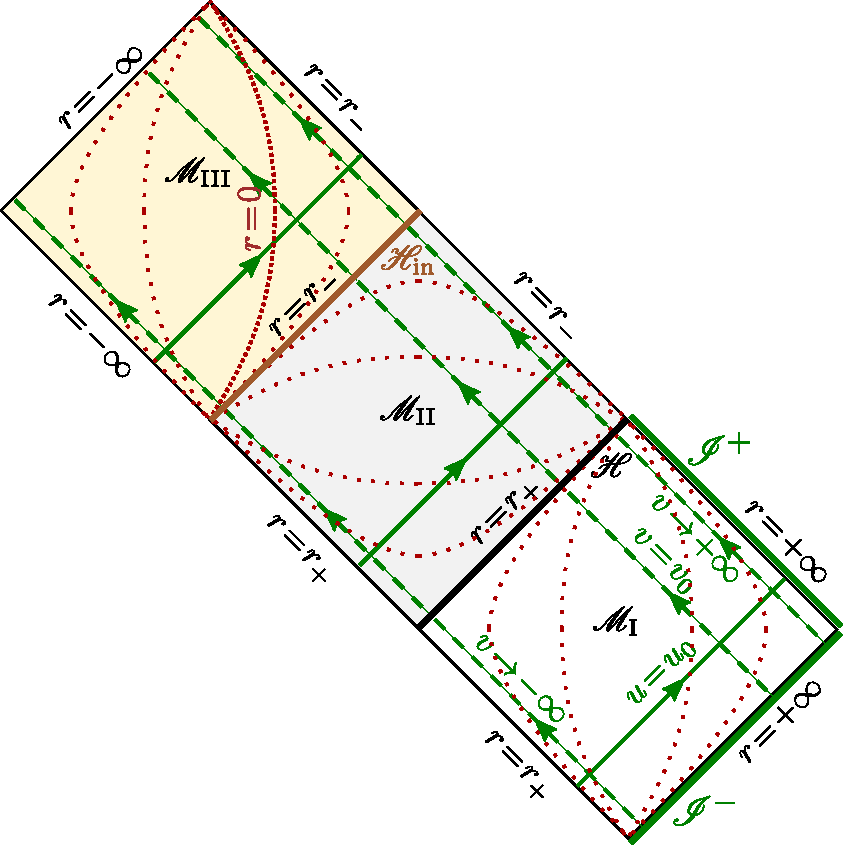
\includegraphics[width=0.6\textwidth]{ker_3blocks_in.pdf}}
\caption[]{\label{f:ker:3blocks_in} \footnotesize
Conformal diagram of the manifold $\M = \R^2\times\SS^2 \setminus \ring$,
defined as the Kerr spacetime in Sec.~\ref{s:ker:Kerr_coord} [Eq.~(\ref{e:ker:def_M_Kerr_spacetime})], spanned by the ingoing principal null geodesics (dahsed green lines). The dotted curves marks the hypersurfaces $r=\mathrm{const}$.}
\end{figure}

\begin{figure}
\centerline{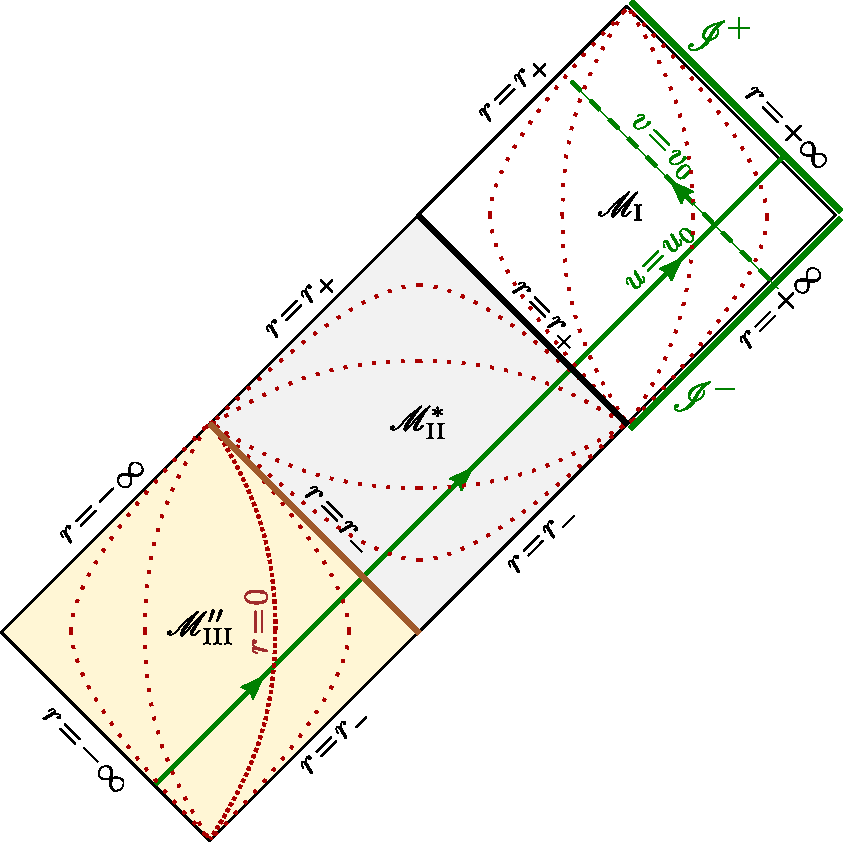
\includegraphics[width=0.6\textwidth]{ker_3blocks_out.pdf}}
\caption[]{\label{f:ker:3blocks_out} \footnotesize
Conformal diagram of the minimal extension of $\M_{\rm I}$ to ensure
complete outgoing principal null geodesics (one of them is drawn as a solid green line).}
\end{figure}

\begin{figure}
\centerline{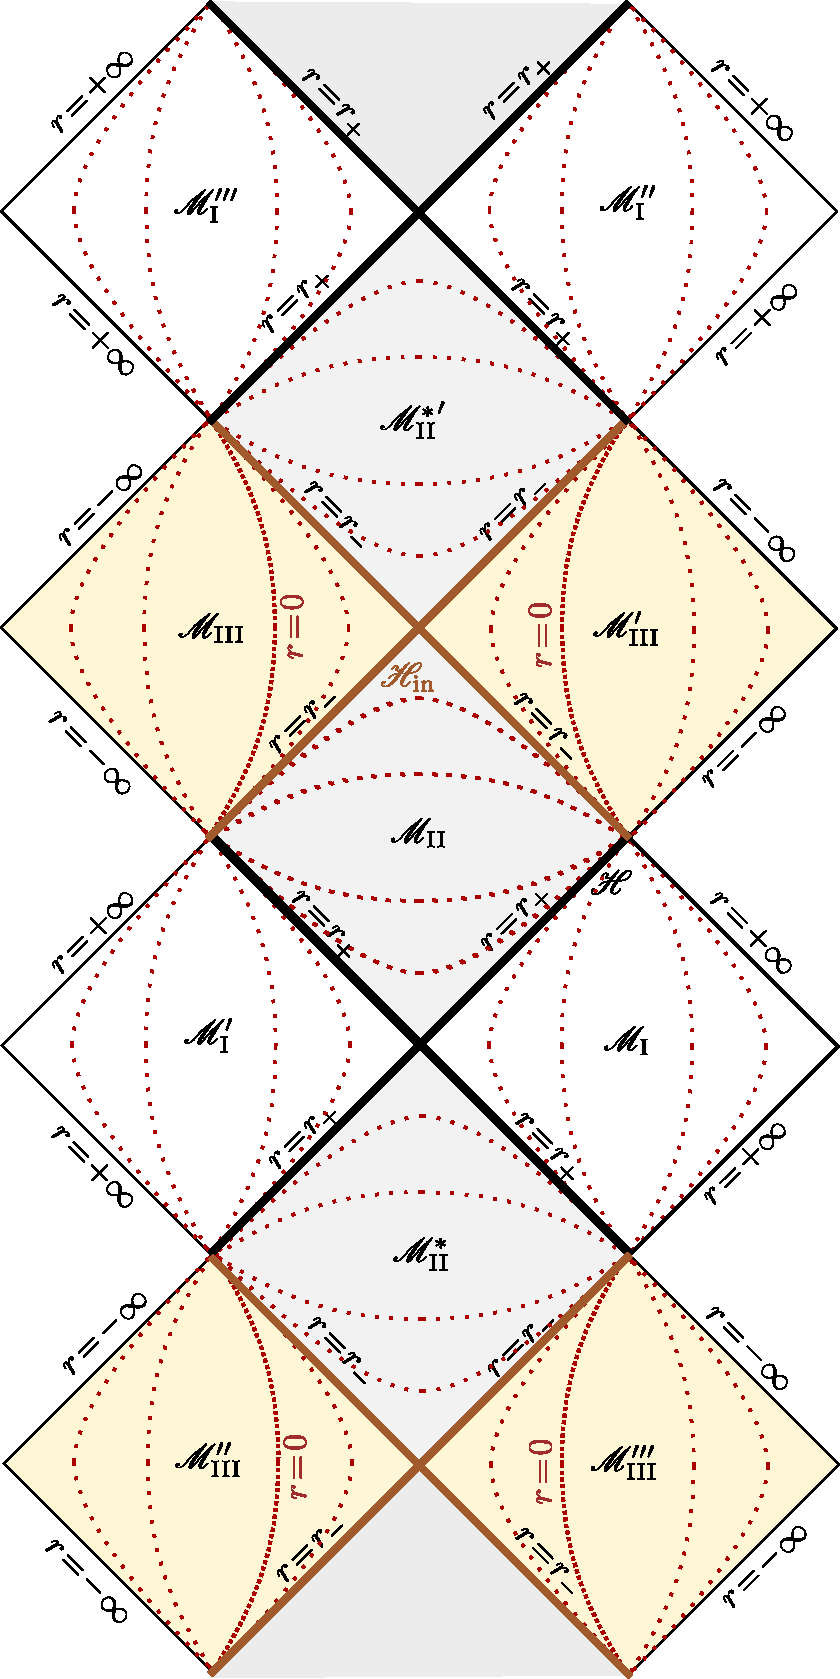
\includegraphics[width=0.6\textwidth]{ker_max_ext.pdf}}
\caption[]{\label{f:ker:max_ext} \footnotesize
Maximal analytic extension of the Kerr spacetime.}
\end{figure}

\subsection{Cauchy horizon}
